\chapter[Paper: Hierarchical Heuristic Search Using A Gaussian Mixture Model for UAV Coverage Planning]{Paper: Hierarchical Heuristic Search Using A Gaussian Mixture Model for UAV Coverage Planning\footnote {Submitted to SMC-B (IEEE Transactions On Systems, Man And Cybernetics Part B, Cybernetics) journal and under 3rd round of review. Authors are Lanny Lin, and Michael A. Goodrich.}}
\label{chap:SMCB2014}

\begin{abstract}
During UAV search missions, efficient use of UAV flight time requires flight paths that maximize the probability of finding the desired subject. The probability of detecting the desired subject based on UAV sensor information can vary in different search areas due to environment elements like varying vegetation density or lighting conditions, making it likely that the UAV will only be partially able to detect the subject. This adds another dimension of complexity to the already difficult (NP-hard) problem of finding an optimal search path. We present a new class of algorithms that account for partial detection in the form of a task-difficulty map and produce paths that approximate the payoff of optimal solutions. The algorithms use the \textit{Mode Goodness Ratio} heuristic, which uses a Gaussian Mixture Model to prioritize search subregions. The algorithms search for effective paths through the parameter space at different levels of resolution. We compare the performance of the new algorithms against two published algorithms (Bourgault's algorithm and LHC-GW-CONV algorithm) in simulated searches with three real search and rescue scenarios, and show that the new algorithms outperform existing algorithms significantly and can yield efficient paths that yield payoffs near the optimal.  
\end{abstract}


%\begin{IEEEkeywords}
%Unmanned aerial vehicles, path planning, navigation, hierarchical systems, heuristic algorithms
%\end{IEEEkeywords}
%
%\IEEEpeerreviewmaketitle

%=================================================================================
\section{Introduction}
\label{sec:Introduction}

%\IEEEPARstart

Mini-UAVs (Unmanned Aerial Vehicles) are becoming useful tools in many reconnaissance, remote-sensing, surveillance, and search operations thanks to advances in UAV technologies. They can help firefighters map forest fires, help news crews provide coverage, help police monitor crowds, and help wilderness search and rescue workers locate a missing person. In these applications, the UAV uses its on-board cameras to provide useful visual information in support of the specific operation.

This paper focuses on using mini-UAVs to support Wilderness Search and Rescue (WiSAR). The aerial view from a UAV enables WiSAR workers to survey large areas of importance in real time~\cite{Goodrich2008Supporting}. Search efficiency is very important in WiSAR because, as time progresses, the survivability of the missing person decreases and the effective search radius increases by approximately 3km/hour~\cite{Syrotuck2000Introduction}. Therefore, a good flight path should rapidly maximize the probability of finding the missing person to make efficient use of the limited flying time.

Each UAV path accumulates information over time as the UAV's sensors scan the ground. As illustrated in Fig.\ref{TwoApproaches}, various paths do so in different ways depending on how information is distributed in the environment. The goal is to maximize the total probability of detection. There are two quality metrics for the probability-maximizing path planning problem~\cite{Koopman1957Theory, Stone1975Theory, Washburn1981Search}. First, find the path that maximizes the Cumulated Detection Probability (CDP) after a specific flight time (blue vertical dotted line). Out of the three example paths in Fig.
\ref{TwoApproaches} path 3 becomes the winner. Second, find the path that achieves a desired CDP in the shortest amount of time (red horizontal dotted line). Path 1 would become the winner out of the three, instead. We model the problem following the first approach.
\begin{figure}
\centering
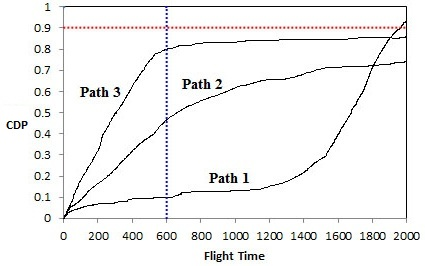
\includegraphics[width=5in]{Approaches.jpg}
\caption{Two approaches to the probability-maximizing path planning problem. With three paths generated by various algorithms, the first approach prefers the path maximizing the Cumulated Detection Probability (CDP) given a specific flight time (Path 3 is the winner) and the second approach prefers the path achieving a specified CDP in the shortest amount of time (Path 1 is the winner)}. 
\label{TwoApproaches}
%\vspace*{-3ex}
\end{figure}

When using a UAV's on-board camera to assist WiSAR operations, factors such as dense vegetation, lighting conditions, shadows, or distance between the camera and the ground can lower the quality of the UAV aerial view and decrease the probability of detection~\cite{Morse2010UAV}. This can be attributed to both sensor and human limitations (such as limited attention span and cognitive workload). We propose to represent \textit{partial detection} in the form of a task-difficulty map, where a more difficult subregion on the map has lower probability of detection. Using a task-difficulty map enables us to integrate geo-referenced and spatial-related sensor constraints into the problem formulation, which supplements traditional sensor modeling methods (e.g.,~\cite{Bourgault2006Optimal}) and potentially improves search performance in real world search scenarios. Because detection difficulties vary in different search subregions, flying patterns such as lawnmower and Zamboni don't guarantee optimal coverage. Integrating the task-difficulty map into path planning adds another dimension of complexity to the already difficult problem and causes the performance of existing greedy-type algorithms (Bourgault's Algorithm~\cite{Bourgault2006Optimal} and LHC-GW-CONV~\cite{Lin2009UAV}) to suffer.

We model the path planning problem as a discrete combinatorial optimization problem, and propose a new heuristic, the \textit{Mode Goodness Ratio}. This heuristic uses a Gaussian Mixture Model to identify and prioritize search subregions. We then present two new algorithms (\textit{Top2} and \textit{TopN}) that utilize the heuristic in hierarchical path planning by forcing the UAV to visit high priority subregions. The hierarchical structure enables the algorithms (a) to cluster probability volumes and (b) to prioritize search subregions at different levels of resolution. It also makes it easy to parallelize the two new algorithms and improve computation speed. We compare the performance of the new algorithms against two published algorithms (Bourgault's Algorithm~\cite{Bourgault2006Optimal} and LHC-GW-CONV algorithm~\cite{Lin2009UAV}) in simulated searches based on three real search and rescue scenarios. Results show that the new algorithms outperform existing algorithms significantly and can yield efficient paths that approximate the payoff of the optimal path.

The contributions of the paper are (a) the introduction of Gaussian Mixture Model (GMM) to compute the Mode Goodness Ratio heuristic, which can be used to prioritize search subregions in a hierarchical planner, (b) two new path planning algorithms that utilize the Mode Goodness Ratio heuristic to improve path-planning performance, and (c) the use of a spatial representation (task-difficulty map) in modeling sensor detection probability with terrain and vegetation information and incorporating that into UAV path planning.

Section~\ref{sec:ProblemFormulation} defines the problem and the metrics used to evaluate algorithm performance. Section~\ref{sec:RelatedWork} discusses related literature. Section~\ref{sec:PathPlanningAlgorithms} first reviews two existing algorithms and then demonstrates the weakness of these algorithms with a synthetic scenario. This section then presents the \textit{Mode Goodness Ratio} heuristic and the two new algorithms (\textit{Top2} and \textit{TopN}). Section~\ref{sec:ExperimentResultsAndAnalysis} compares algorithm performance with three real search and rescue scenarios. Section~\ref{sec:LimitationsAndDiscussion} discusses the limitations of the approach, and Section~\ref{sec:Summary} presents the summary.


%=================================================================================
\section{Problem Formulation}
\label{sec:ProblemFormulation}

%=============================
\subsection{Problem Framework}

Typical UAVs (fixed-wing or rotorcraft) are highly mobile and variable, but we will assume a set of useful constraints on their capabilities: they have a gimbaled camera, can maintain a constant height above ground and can travel at constant speed. A gimbaled camera enables the camera to aim straight down even when the UAV is performing roll or yaw maneuvers. We assume that the UAV's speed is much higher than the speed of the missing person and treat the missing person as stationary. At every UAV flight time step, we treat the camera footprint of the search area as a glimpse. This way we can discretize the search area, and model the UAV path planning problem as a discrete combinatorial optimization problem with respect to probability accumulated and define it following the framework described in~\cite{Trummel1986Technical}.

The search space is represented as a finite, connected graph $G = (V, E)$. $V$ denotes the set $\{v_1, ..., v_n\}$ of vertices of $G$, and $E$ denotes the set of edges. Each edge in $E$ can be viewed as an unordered pair of vertices $\{v_i, v_j\}$. The missing person is located at one of the vertices of $G$. A given probability distribution map for the missing person is discretized to match graph $G$, with $p_i$ being the probability that the missing person is located at vertex $v_i$. It is obvious that
\begin{equation}
\sum_{i=1}^{n}p_i = 1.
\label{totalP}
\end{equation}

The UAV search is conducted in discrete time. During each time step, the UAV camera footprint can cover one vertex. For a desired flight with $T$ time steps, let $S$ denote the set $\{0,1,2,...,T\}$. The UAV's motion is constrained by the structure of the graph $G$. Let $\Psi$ be the set of functions $\psi:S \mapsto V$ with the property that for any two consecutive integers $t$ and $t+1$ in $S$, either $\psi(t)=\psi(t+1)$ or $\{\psi(t),\psi(t+1)\}\in E$. Here $\Psi$ represents all possible paths, and under path $\psi$, vertex $\psi(t)$ is searched during step $t$. The conditions on the set $\Psi$ guarantee that at each time step the UAV camera footprint will either remain at the current vertex (only possible for a rotorcraft) or move to a neighboring vertex.

Even when the UAV camera footprint covers the vertex occupied by the missing person, it is not certain that a detection will occur. The probability of detection is described by a glimpse probability function $g$, which is defined by a given task-difficulty map. The task-difficulty map is a spatial representation of sensor detection probability and defines areas where it is difficult to detect the missing person (with lower probability of detection), with $d_i$ being the task-difficulty level at vertex $v_i$. Let $d_{max}$ be the maximum task-difficulty level in the given map. If at time step $t$ the UAV camera footprint covers vertex $v$, then let $g(v,t)$ be the probability that a detection will occur, given that the missing person is at vertex $v$. We model this as
\begin{equation}
g(v_i,t) = 1 - \frac{d_i}{d_{max}+1}.
\label{g}
\end{equation}
so that more difficult tasks (higher $d_i$ values) have lower glimpse detection values, $g$.

Let $P_T(\psi)$ represent the Cumulative Detection Probability (CDP) for path $\psi \in \Psi$ with $T$ time steps. For each (cell, time) pair $(i,t)$ with $1 \leq i \leq n$ and $0 \leq t \leq T$, we define the probability of failure $f(i,t,\psi)$ by 
\begin{equation}
f(i,t,\psi) = 
	\left\{
	\begin{array}{ll}
		1-g(v_i,t) & \mbox{if~} \psi(t)=v_i \\
		1 & \mbox{otherwise.}
	\end{array}
	\right.
\label{OneVertex}
\end{equation}
Let $D_j$ represent a detection on the $j$th observation so $\overline{D}_j$ is a detection failure. Then the probability of failing to detect the the missing person after $N$ observations of vertex $v_i$ given the missing person is at vertex $v_i$ is the joint probability $P(\overline{D}_1, \overline{D}_2, ..., \overline{D}_N|v_i)$. Assuming each observation is conditionally independent of each other (typical in the WiSAR literature), we can rewrite the joint probability as
\begin{equation}
P(\overline{D}_{1:N}|v_i) = \prod_{j=1}^{N}P(\overline{D}_j|v_i),
\label{NoDetection}
\end{equation}
and the probability of detecting the missing person after $N$ observations is
\begin{equation}
P(D_{1:N}|v_i) = 1 -  P(\overline{D}_{1:N}|v_i),
\label{Detection}
\end{equation}
which is equivalent to
\begin{equation}
P(D_{1:N}|v_i) = 1 -  \prod_{t=0}^{T}f(i,t,\psi),
\label{Detection2}
\end{equation}
where $N$ is how many times $v_i$ shows in path $\psi$. Then $P_T(\psi)$ can be computed by
\begin{equation}
P_T(\psi) = \sum_{i=1}^{n}p_i\Big(1 - \prod_{t=0}^{T}f(i,t,\psi)\Big),
\label{CDP}
\end{equation}
where $p_i$ is the probability that the missing person is located at vertex $v_i$. Define $\exists\psi^* \!{\in} \Psi$ such that for any alternate path $\psi' \!{\in} \Psi, P_T(\psi^*) \!{\geq} P_T(\psi')$. Our goal is to find the optimal path $\psi^*$ that produces the maximum CDP (path 3 in~Fig.\ref{TwoApproaches} at $T=600$ if there are only three possible paths) or find an efficient path $\psi'$ that produces payoff approximating the payoff of the optimal path within reasonable computation time.

When the path needs to end at an operator-specified vertex (for easy UAV retrieval or to join with other path segments), we simply add the constraint to the problem formulation (only add edges to a path that does not violate the constraint so the UAV has enough time to reach the end point). Also for fixed-wing UAVs, additional motion constraints (such as not allowing the UAV to fly backward) are also introduced as velocity constraints affecting edges $\{\psi(t), \psi(t_1)\}$, effectively creating a directed graph. Both proposed path planning algorithms satisfy these constraints.

%=============================
\subsection{Performance Metrics}

%Let $\mathit{Efficiency_{LB}}$ (Efficiency Lower Bound) and algorithm Run Time producing path $\psi'$ denote metrics to measure the performance of the algorithms. 
We will use two measures of algorithm performance: the quality of the path and the run-time of the algorithm. Run-time is self-explanatory, but we need a measure of path quality. Ideally the efficiency of an algorithm should be computed with the following equation:
\begin{equation}
\mathit{Efficiency}(\psi') = \frac{P_T(\psi')}{P_T(\psi^*)},
\label{Efficiency}
\end{equation}
where $\psi^*$ is the optimal path. However, because we do not know what $\psi^*$ is, we bound the efficiency. Let $\psi_{teleport}$ be defined as the path constructed as follows: (a) deduct the time needed to move from the start vertex to the nearest vertex with non-zero $p_i$ (plus time for doing the same with the end vertex if specified), and (b) at each step the UAV teleports to the vertex that allows the UAV to collect the highest amount of probability after considering the task-difficulty at that vertex. Then, all the probability collected during the teleport flight is summed, giving $\mathit{Efficiency_{LB_i}}$ for path $i$:
\begin{equation}
\mathit{Efficiency_{LB_i}} = \frac{P_T(\psi_i)}{P_T(\psi_{teleport})}
\label{EfficiencyLB}
\end{equation}
Since $P_T(\psi^*) \leq P_T(\psi_{teleport})$, $\mathit{Efficiency}$ can be no worse than $\mathit{Efficiency_{LB}}$, so the latter sets a lower bound for the true efficiency. Note that the majority of the teleport path $\psi_{teleport}$ is made up of disjointed points because the UAV would be ``jumping'' (teleporting) from vertex to vertex, always landing on the vertex that promises highest amount of probability collectable.

%=================================================================================
\section{Related Work}
\label{sec:RelatedWork}

Many path planning algorithms in the literature address obstacle avoidance while planning a path to reach a destination using A*~\cite{Quigley2005Towards}, D*~\cite{Stentz1997Optimal}, Voroni diagrams~\cite{Bortoff2000Path}, or probability roadmaps and rapidly-exploring random tree (RRTs)~\cite{Pettersson2006Probabilistic}. Hierarchical heuristics approaches were also developed, such as Hierarchical A* (HA*) by Holte et al.\ ~\cite{Holte1996Hierarchical}, hierarchical task-based real-time path planning by Naveed et al.\ ~\cite{Meuleau2007Hierarchical}, and Hierarchical-AO* (HiAO*) by Meuleau and Brafman~\cite{Naveed2010Hierarchical}. The algorithms we present solve a different path planning problem by generating paths that make efficient use of the limited travel time and maximizing the probability of finding the missing person. This is similar to the Vehicle Routing Problem~\cite{Laporte1992Vehicle} and the Orienteering Problem (OP), which is a variation of the Traveling Salesman Problem (TSP) and is known to be NP-Hard~\cite{Sokkappa1990Cost}. However, our path planning problem is even more difficult with added challenges of repeated visits and partial detection. 
%A good analogy would be thinking of the UAV as a vacuum cleaner sucking up probabilities as it flies over a search area. However the sucking efficiency might vary from carpet to hardwood floor. 
Tasgetiren and Smith propose a Genetic Algorithm in~\cite{Tasgetiren2000Genetic} to solve OP. Liang and Smith present an Ant Colony Optimization approach that uses an unusual sequenced local search and a distance-based penalty function for path planning~\cite{Liang2006Ant}. These algorithms work well with OP problems with few nodes (21--100) but can be slow with many nodes. Unfortunately, they do not allow repeated visits and do not support partial detection. Although classic dynamic programming~\cite{sniedovich2010dynamic} method can solves TSP, because TSP is NP-hard, it cannot be solved in polynomial time, unless P=NP. The method suffers the ``curse of dimensionality'' and does not scale well with complex problems. Reinforcement learning (approximate dynamic programming) methods~\cite{Bertsekas1995Dynamic,Sutton1998Reinforcement} have four main sub-elements: a policy, a reward function (immediate payoff), a value function (long-term payoff), and optionally, a model of the environment. Because in our path planning problem, a node can be visited multiple times, and because our Bayesian approach allows for partial collection of information, the score/prize collected for each visit is different. The reward function and the value function both become path dependent, the state space becomes exponentially large. We seek a real-time solution that scales well when search area and flight duration expand, therefore we prefer a heuristic approach.

In the 1950's, Koopman discussed the uncertainties in the act of detecting hostile submarines with radars and proposed a concept called the instantaneous probability of detection by one glimpse~\cite{Koopman1956Theory}. He presented simple search algorithms and demonstrated how search effort should be distributed given a prior probability distribution of the target and known law of detection when only a limited total amount of search effort (or time) is available~\cite{Koopman1957Theory}. Stone~\cite{Stone1975Theory} presents various search plans with partial detection models using Lagrange multipliers and maximization of Lagrangians in finding stationary target in very basic search problems when no false targets are present. Washburn~\cite{Washburn1981Search} discusses how to construct optimal search paths for different search problems. The author also developed detection models based on radar/sonar and expanded the fundamentals of search theory to include moving targets. In~\cite{Bourgault2006Optimal} Bourgault et al.\ describe a Bayesian framework for UAV trajectory planning to maximize the chances of finding the target given restricted time. Partial detection was modeled based on a downward-looking millimeter wave radar, and a one-step lookahead method was used for path planning using posterior distributions obtained from Bayes filter~\cite{Thrun2005Probabilistic} updates. More recent work includes~\cite{Niedfeldt2010integrated} where Niedfeldt et al.\ present a UAV path planning algorithm that utilizes probability of detection and maximizes the probability of identifying an object using a N-step lookahead method, and~\cite{Ryan2010particle} where Ryan and Hedrick developed a control formulation for a fixed-wing UAV that minimizes the entropy of an estimate distribution over a receding horizon for searching a moving target over a fixed time horizon. N-step lookahead and receding horizon methods are greedy-type algorithms that run into scalability bounds and generate sub-optimal paths in situations when a complicated detection model is used, such as a task-difficulty map.

Koester compiled statistics from large set of past WiSAR incidents~\cite{Koester2008Lost}. These statistics can be used to construct probability distribution maps. Ferguson describes how GIS can be used to segment search areas into probability subregions~\cite{Ferguson2008GIS}. Goodrich et al.\ ~\cite{Goodrich2008Supporting} describe how a probability distribution of likely places to find the missing person can be useful for UAV path planning. Lin and Goodrich~\cite{Lin2010Bayesian} propose a Bayesian model to create such a distribution based on terrain features and past human behavior data. The model has been evaluated using real search and rescue scenarios at George Mason University's MapScore web portal~\cite{Twardy2012MapScore}
%\footnote{George Mason University's MapScore Lost Person Model Rating System by Dr. Charles Twardy at http://mapscore.sarbayes.org:8000/main/}
and performed well compared to other statistical models. Stone et al.\ used posterior probability maps and successfully located the wreckage of Air France Flight 447~\cite{Stone2011Search}. Metrics such as Koopman's instantaneous probability of detection by one glimpse~\cite{Koopman1956Theory}, ``seeability'' proposed by Morse et al.\ \cite{Morse2010UAV}, and terrain and vegetation information obtained from USGS~\cite{Lin2010Bayesian} can be used to build a task-difficulty map representing probability of detection in different search subregions.

The \textit{Mode Goodness Ratio} heuristic is used to evaluate the ``peakedness'' of a bivariate Gaussian. The traditional way to evaluate the peakedness of a distribution uses kurtosis~\cite{Balanda1988Kurtosis}. Mardia~\cite{Mardia1970Measures} extends the concept to multivariate distributions. Because multivariate kurtosis is difficult to compute and may show inconsistency in the meaning the peakedness
of a distribution, Khurshid et al.\ ~\cite{Khurshid2007Note} extend Horn's measure of peakedness~\cite{Horn1983Measure} into a measure for bivariate normal distributions. The heuristic we propose is an even simpler method to measure the peakedness and is well-adapted to support hierarchical search algorithms.

%=================================================================================
\section{Path Planning Algorithms}
\label{sec:PathPlanningAlgorithms}

In this section we review two existing path planning algorithms, Bourgault's Algorithm~\cite{Bourgault2006Optimal} (referred to as BA from here on) and LHC-GW-CONV~\cite{Lin2009UAV}, and demonstrate the weakness of these algorithms with a synthetic scenario. Next we formally define the Mode Goodness Ratio heuristic. Then we present the Top2 \& TopN algorithms.

%=============================
\subsection{BA and LHC-GW-CONV algorithms review}
\label{BALHCReview}


The BA algorithm~\cite{Bourgault2006Optimal} is a Bayesian approach to the UAV path planning problem. Given a prior probability distribution of the missing person, it uses the Bayes filter as described in~\cite{Thrun2005Probabilistic} to compute the posterior probability distribution at every time step. 
%The Bayes filter includes a prediction step (Equation~\ref{prediction}) and an update step (Equation~\ref{update}) using the UAV's sensor observation. 
The probability of detection follows an active model of a downward looking millimeter wave radar where signal power is determined by factors such as emitted power, antennae footprint, and sensor distance to the target. Distributions are discretized into a grid for calculation and a (greedy) one-step lookahead method is used to determine which cell the UAV should fly to next (the grid cell with the highest posterior probability). 
%In Equation~\ref{prediction} and~\ref{update}, $\textbf{x}_k^t$ is the probability distribution of the target $t$ at time $k$; this is equivalent to the graph $G$ we defined in Section~\ref{sec:ProblemFormulation} where $p_i$ is the probability that the missing person is located at vertex $v_i$. $p(\textbf{z}_k|\textbf{x}_k^t)$ is the probability of detection, and is similar to $g(v_i,t)$ in Equation~\ref{OneVertex}.
%\begin{equation}
%p(\textbf{x}_k^t|\textbf{z}_{1:k-1}) = \int{p(\textbf{x}_k^t|\textbf{x}_{k-1}^t|\textbf{z}_{1:k-1})d\textbf{x}_{k-1}^t}
%\label{prediction}
%\end{equation}
%\begin{equation}
%\begin{split}
%p(\textbf{x}_k^t|\textbf{z}_{1:k}) &= Kp(\textbf{x}_k^t|\textbf{z}_{1:k-1})p(\textbf{z}_k|\textbf{x}_k^t), \\
%\mbox{~~where~~} K &= 1 / \int{[p(\textbf{x}_k^t|\textbf{z}_{1:k-1})p(\textbf{z}_k|\textbf{x}_k^t)]d\textbf{x}_k^t}
%\end{split}
%\label{update}
%\end{equation}

Our formulation in Section~\ref{sec:ProblemFormulation} can be viewed as a Bayes filter with the following assumptions: $p_i$ is the prior probability, $g(v_i,t)$ is the detection likelihood, and we assume a stationary object of interest. Instead of using a greedy approach, we look ahead much further down the path. In order to address the increased computational complexity, we use a heuristic (introduced in the next section) and rely on a hierarchical approach to improve the search for efficient paths. Because the speed of our algorithms is very fast, our algorithms can turn into a ``greedy'' algorithm with extended horizon when dealing with moving object or changing environment.

The sensor model in BA uses target distance and signal strength, which implicitly considers the spatial information of the environment. We use a task-difficulty map to take advantage of explicit prior knowledge of the environment and how it affects the detection probability spatially. For a fair comparison, we used the same downward-looking camera visual sensor model when we implemented the BA algorithm, and we note that our algorithm can use detection models similar to the one used in~\cite{Bourgault2006Optimal}.

The LHC-GW-CONV algorithm~\cite{Lin2009UAV} is a combinatorial optimization approach to the UAV path planning problem. It discretizes the given probability distribution of the missing person and the task-difficulty map into a grid and uses a Local Hill-Climbing algorithm to select the next cell to fly to (the grid cell with the highest one glimpse detection probability). Spatial averaging is performed by convolving the combined probability distribution and the task-difficulty map using box filters. This serves as the tie-breaker, enabling the algorithm to look beyond local neighbors in order to plan paths toward broader areas with high probability. Even with spatial smoothing a typical problem of LHC is that it favors local maxima, resulting in the UAV getting stuck in a local probability hill for too long before it can move to another probability hill. To overcome the problem, a ``Global Warming'' technique is used\footnote{The name ``Global Warming'' comes from the metaphor where the ``ocean surface'' represents all the grid cells with zero probability and the ``islands'' represent probability hills with non-zero grid cells; as the ``ocean'' rises the volume of probability hills above the water decreases.}. After each ``ocean rise'', a new path is created, and the best path is returned as the final path found. Equation~\ref{GW} shows how the probability $p_i$ that the missing person is at vertex $v_i$  changes when the ``ocean'' rises.
\begin{equation}
p_i' \leftarrow
	\left\{
	\begin{array}{ll}
		p_i - nC, & \mbox{if~~} p_i > nC \\
		0, & \mbox{otherwise}
	\end{array}
	\right.
\label{GW}
\end{equation}
where $C$ is a constant height of each ``ocean rise'' and $n$ is how many times the ``ocean'' will rise.

Both BA and LHC-GW-CONV are greedy algorithms. The advantages of greedy algorithms include low computational cost and flexibility in quickly adapting to changes (e.g., a changing environment or a moving target). A major drawback is that such algorithms tend to get stuck in local maxima. We can demonstrate this using the synthetic scenario in Fig.\ref{SyntheticCase}, which shows a multi-modal distribution of the missing person location and a simple task-difficulty map with three difficulty levels. 

For a UAV path where $T=900$, if the UAV starts from a subregion with low task-difficulty (upper left corner), the BA algorithm achieved 65.99\% $\mathit{Efficiency_{LB}}$ and the LHC-GW-CONV algorithm achieved 96.28\% (averaged for 10 runs); Fig.\ref{SyntheticCasePaths1} shows the paths generated by the two algoirthms. The BA algorithm's performance is okay but not great, while the LHC-GW-CONV algorithm performed really well (actually slightly better than the performance of the Top2 and TopN algorithms, which we will discuss in detail in section~\ref{sec:LimitationsAndDiscussion}). But if the UAV starts from a subregion with high task-difficulty (lower right corner), both algorithms perform poorly (much worse than the performance of the Top2 and TopN algorithms), with BA scoring 41.91\% and LHC-GW-CONV scoring 53.71\% (averaged for 10 runs) in $\mathit{Efficiency_{LB}}$; Fig.\ref{SyntheticCasePaths2} shows the paths generated by the two algoirthms. This is because both greedy algorithms fail to move the UAV quickly out of the local probability hill. The Top2 and TopN algorithms we propose address this problem by forcing the UAV to visit other search subregions and also allocate more flight time to subregions where the UAV can be more efficient. In order to identify better subregions, we propose the Mode Goodness Ratio heuristic.
\begin{figure}
\centering
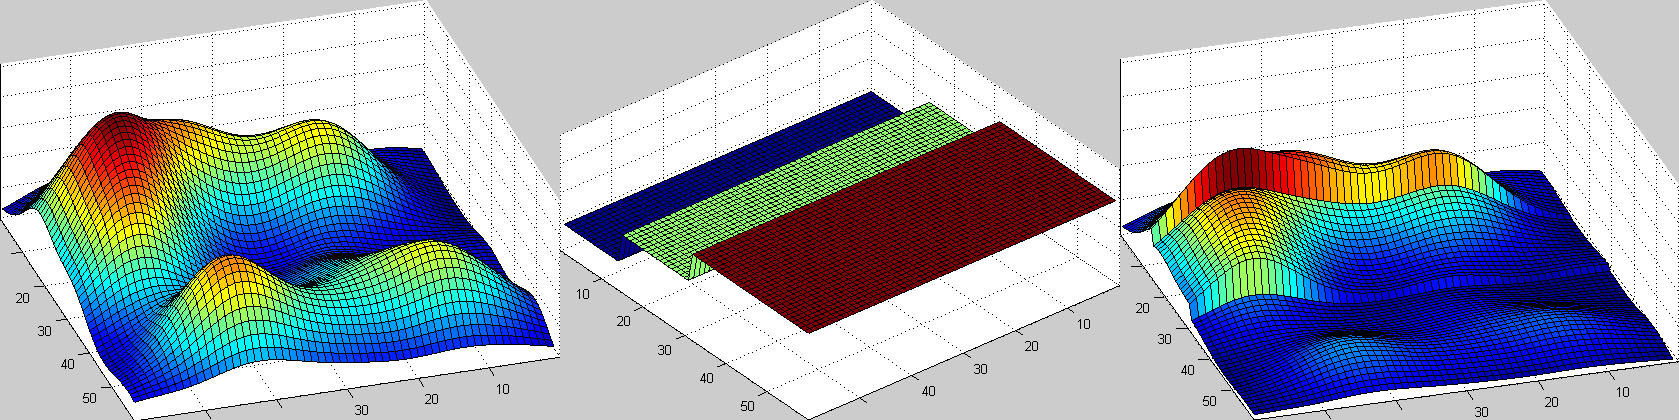
\includegraphics[width=6in]{Multimodal1.jpg}
\caption{A synthetic WiSAR scenario. Left: Multi-modal probability distribution. Middle: A simple task-difficulty map. Right: Probability collectible on first visit (combining probability distribution and task-difficulty map).}
\label{SyntheticCase}
%\vspace*{-1ex}
\end{figure}

\begin{figure}
\centering
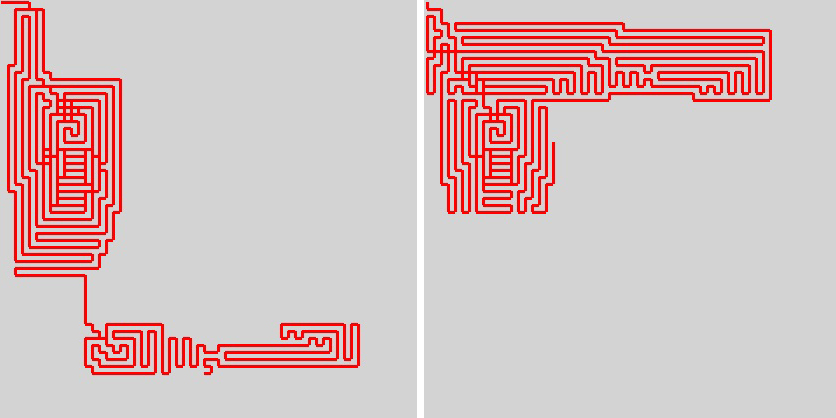
\includegraphics[width=5in]{TestCaseTopLeft.jpg}
\caption{Paths found at $T=900$ when the UAV starts from a subregion with low task-difficulty (upper left corner). Left: Path created by BA. Right: Path created by LHC-GW-CONV.}
\label{SyntheticCasePaths1}
%\vspace*{-3ex}
\end{figure}

\begin{figure}
\centering
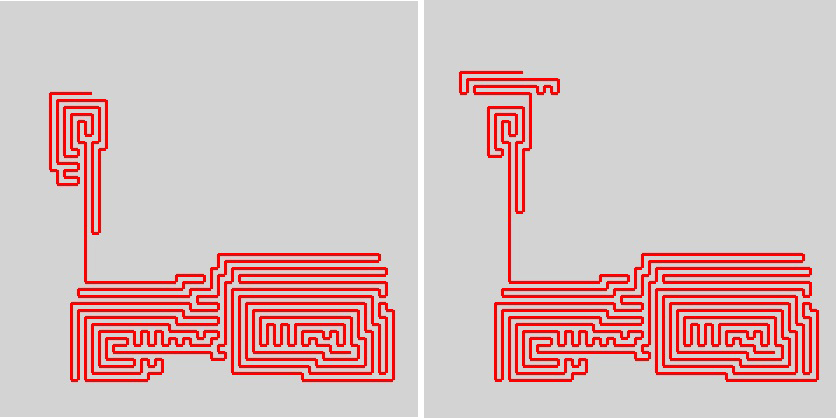
\includegraphics[width=5in]{TestCaseBottomRight.jpg}
\caption{Paths found at $T=900$ when the UAV starts from a subregion with high task-difficulty (lower right corner). Left: Path created by BA. Right: Path created by LHC-GW-CONV.}
\label{SyntheticCasePaths2}
%\vspace*{-3ex}
\end{figure}

%=============================
\subsection{Mode Goodness Ratio}

The Mode Goodness Ratio heuristic prioritizes search subregions, where each subregion represents a cluster of probability volume that can be ``collected'' by the UAV sensor. Compute the heuristic as follows: First, combine the probability distribution map and the task-difficulty map to construct a new grid/surface $G'$. The value of each cell in $G'$ represents how much probability can be collected the first time the cell is visited (e.g., the right part of Fig.\ref{SyntheticCase}). Second, use a Gaussian Mixture Model (GMM) to partition $G'$ into high quality clusters/subregions. We subjectively set the maximum number of subregions to 5 to reduce computational complexity.
%($1\!{<}k\!{\leq}5$)\footnote{Note that probability models for missing person location in a manageable search area are unlikely to be at high enough resolution to exceed this threshold; see section~\ref{sec:ExperimentResultsAndAnalysis}}.

A GMM is a probabilistic model for finding sub-populations within an overall population and is often used for data clustering. We choose the GMM method for two reasons: 1) We can take advantage of the resulting Gaussian parameters and coefficients to estimate the peakedness of the probability hills. 2) A GMM is a parametric method, so we can define subregions by cluster probability volume hierarchically and search through the parameter space.

It is important to point out that when a task-difficulty map (especially a complicated one) is applied, the resulting grid/surface $G'$ is unlikely to resemble a mixture of Gaussians and we only use GMM to approximate the probability hills.

We used the Accord.MachineLearning library in the Accord.NET framework\footnote{http://code.google.com/p/accord/} to estimate GMM parameters. We generate data points to approximate $G'$ (create a 2D histogram of $G'$ and generate number of points proportional to each bin count) and then feed these points to the Accord library, which first uses the K-Means algorithm to generate $k$ initial clusters, and then uses the Expectation Maximization (EM) algorithm to iteratively fit data to a mixture of Gaussians. Gupta and Chen provide detailed description on how to use EM to learn a GMM model in~\cite{Gupta2011Theory}. The results are a set of ($k$) scaled Bivariate Gaussian distributions with their means, covariance matrices, and the coefficient (scale) for each Gaussian. For completeness, Equation~\ref{multivariate} shows the density function for a multivariate Gaussian distribution.
\begin{equation}
P(\mathbf{x}) = \frac{1}{\sqrt{(2\pi)^n|\mathbf{\Sigma}|}} e^{-\frac{1}{2}\left( (\mathbf{x}-\mathbf{\mu})^{\top}\mathbf{\Sigma}^{-1} (\mathbf{x}-\mathbf{\mu}) \right)} ,
\label{multivariate}
\end{equation}

Next we identify all modes in the grid/surface $G'$ (using simple local hill-climbing with verification for plateaus and ridges), and match the mean of each Gaussian to the closest mode centroid (in case the mode has a flat peak) and then use that centroid, $C_i$, to represent the subregion. Note that the number of modes in $G'$ can be more than the number of modes in the probability distribution after a task-difficulty map is applied. If there are fewer than 5 modes in $G'$, we reduce $k$ accordingly to reduce computation.

We evaluate three factors when computing Mode Goodness, $MG_i$, for subregion $i$: distance ratio $D_i$, probability volume $V_i$, and subregion area $A_i$. 

The first factor, the \textit{distance ratio} $D_i$, is defined as:
\begin{equation}
D_i = \log\Big(\frac{T}{\alpha_i+1}\Big),
\label{DistanceRatio}
\end{equation}
where $T$ is the total UAV flight time (in time steps) and $\alpha_i$ is the L1 norm distance from the start location of the path to the centroid of the subregion, $C_i$. If an end location is specified for the path, then that distance is also added:
\begin{equation}
\alpha_i = 
	\left\{
	\begin{array}{ll}
		||\mbox{Start}-C_i||_1, & \mbox{no End} \\
		||\mbox{Start}-C_i||_1 + ||\mbox{End}-C_i||_1, & \mbox{otherwise}
	\end{array}
	\right.
\label{Alpha}
\end{equation}
We add 1 to the denominator in Equation~\ref{DistanceRatio} to make sure it will never be 0, and use the log scale to reduce wide-ranging quantities to a smaller range. 

The idea behind the distance ratio is that a subregion is less attractive when it takes a large percentage of the total flight time to reach the center of the subregion because the trip to get there might not be very efficient. Therefore, higher $D_i$ values indicate closer subregions.

The second factor, the \textit{probability volume} $V_i$, is defined as:
\begin{equation}
V_i = V_{3\sigma_{x'_i}3\sigma_{y'_i}}w_i,
\label{Volume}
\end{equation}
where $V_{3\sigma_{x'_i}3\sigma_{y'_i}}$ is a constant (roughly 99.46\%) representing the volume of probability under a standard bivariate Gaussian surface within 3 standard deviations, and $w_i$ is the weight of each Gaussian component $G_i$, which is the coefficient of the Gaussian in the mixture as shown below with the property of $\sum_{i=1}^k w_i = 1$.
\begin{equation}
p(\mathbf{x}) = \sum_{i=1}^k w_i G_i
\label{Alphas}
\end{equation}
The idea behind the probability volume is that a subregion is more attractive when the volume of probability within the subregion is high, meaning visiting the subregion has the potential of collecting a large amount of probability. Therefore, higher $V_i$ values indicate subregions with more probability.

After rotating the axes of the bivariate Gaussian to align with the eigenvectors of the covariance matrix $\mathbf{\Sigma}_i$, the area under the surface within 3 standard deviations in both axes can be estimated using a rectangle with width $3\sigma_{y'_i}$ and height $3\sigma_{x'_i}$ where $\sigma_{x'_i}$ and $\sigma_{y'_i}$ are the square roots of the eigenvalues of the Gaussian's covariance matrix. The \textit{area} of the rectangle $A_i$ is the third factor in the heuristic. A larger $A_i$ means it takes more time steps for a UAV to cover the area. Therefore, the lower $A_i$ is, the better the subregion.
\begin{equation}
A_i = (3\sigma_{x'_i})(3\sigma_{y'_i}) = 9\sigma_{x'_i}\sigma_{y'_i}.
\label{Area}
\end{equation}

When we divide $V_i$ by $A_i$, we are basically estimating the peakedness of the Gaussian. Then assuming the peakedness is independent of the distance ratio $D_i$, we can multiply them together to compute the Mode Goodness of the subregion $i$:
\begin{equation}
MG_i = D_i V_i {A_i}^{-1}.
\label{Goodness}
\end{equation}

Since all we really care about is the priority order of the search subregions, we can simplify computation by computing the Mode Goodness Ratio, $\mathit{MGR}_i$, for subregion $i$ with respect to subregion 1 as the following:
\begin{align}
\mathit{MGR}_i &= \frac{MG_i}{MG_1} = \frac{D_i V_i {A_i}^{-1}}{D_1 V_1 {A_1}^{-1}} \\
&= \frac{D_i V_{3\Sigma} S_i (9\sigma_{x'_i}\sigma_{y'_i})^{-1}}{D_1 V_{3\Sigma} S_1 (9\sigma_{x'_1}\sigma_{y'_1})^{-1}} \\
&= \frac{D_i S_i (\sigma_{x'_i}\sigma_{y'_i})^{-1}}{D_1 S_1 (\sigma_{x'_1}\sigma_{y'_1})^{-1}}
\label{GoodnessRatio}
\end{align}

Naturally, $\mathit{MGR}_1$, the Mood Goodness Ratio for subregion 1 with respect to subregion 1 will always be 1 and $\mathit{MGR}_i$ for other subregions can be less or greater than 1. By sorting the Mode Goodness Ratios of all the subregions, we have a way of prioritizing them according to their mode goodness.


%=============================
\subsection{Top2 Algorithm}

The Top2 algorithm is designed to generate paths that force the UAV to visit the top 2 subregions in the search area. This way the heuristic-based path planner can escape from a probability hill where task-difficulty is high and probability of detection is low. First the Mode Goodness Ratio heuristic is used to identify the top 2 search subregions (represented by centroids). Then, local hill climbing is used to create the shortest path segment from the start location to the nearest centroid. If an end location is specified in the path planning request, another path segment is created similarly from the end location to the other centroid. 

The algorithm then identifies a point (vertex) equidistant from the two centroids (the green square) and launches two path planning tasks to plan path segments from each centroid to that point using local hill climbing. By allocating different percentages of the remaining flight time to these two path planning tasks, the Top2 algorithm can effectively search within a new dimension of time allocation. The subregion with more flight time allocated ends up with a longer path segment. Note that it is possible for the path to cover other subregions (other than the top 2) when a lot of flight time is allocated. Fig.\ref{Top2} shows three time allocation examples. 

A coarse-to-fine search is performed starting from a low resolution (large chunks of flight time transfered from one path planning task to the other) and gradually increasing the resolution (smaller chunks) until the best path is found. Then the path segments are joined together to form a full flight path. Fig.\ref{Code1} shows the pseudo-code for the Top2 algorithm.

Because we can specify how many Gaussians to fit during the GMM step, we can actually cluster the probability hills hierarchically, and this structure enables us to search through different hierarchy layers with different $k$ values (e.g., top 2 out of 5, top 2 out of 4, etc.). These path planning tasks at different layers can each run the Top2 algorithm in parallel, taking advantage of the computing power of a multi-processor system; the path with the best performance is returned as the final result.
\begin{figure}
\centering
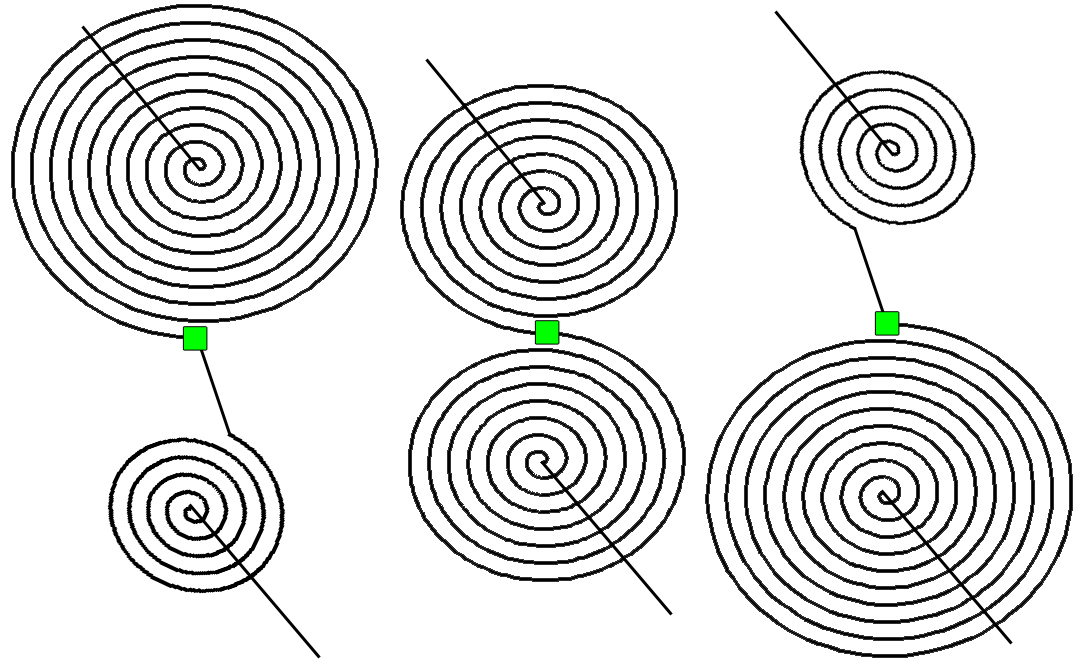
\includegraphics[width=5in]{Top2.jpg}
\caption{Illustrations of the Top2 algorithms where the top is subregion 1 and the bottom is subregion 2. Left: More flight time allocated to subregion 1. Middle: Equal flight time allocated to both subregion 1 and 2. Right: More flight time allocated to subregion 2.}
\label{Top2}
%\vspace*{-3ex}
\end{figure}

\begin{figure}
\noindent\fbox{%
\begin{minipage}{\dimexpr\linewidth-2\fboxsep-2\fboxrule\relax}
%\begin{algorithmic}[1]
Path Top2(Point start, int T, ArrayList centroids, ProbabilityMap map, int tChunk) \{ \\
\setlength\parindent{20pt}
1. Find closest centroid to start c1 and time needed t1  \\
2. Plan straight path from start to c1 and store in path1 \\
3. Find point center equidistant from c1 and c2 \\
\indent map.VacuumProbability(path1); \\
\indent t2min = L1dist(c1, center); \\
\indent t3min = L1dist(c2, center); \\
\indent double efficiency = 0; \\
\indent int t2 = T-t1-t3min; \\
\indent int t3 = T-t1-t2; \\
\indent while (t2 $\geq$ t2min) \{  \\
\indent \indent t2 -= tChunk;\\
\indent \indent t3 += tChunk;\\
\indent \indent (e2, path2) = LHC(c1, center, t2); \\
\indent \indent (e3, path3) = LHC(c2, center, t3); \\
\indent \indent if (e2 + e3 $>$ efficiency) \{ \\
\indent \indent \indent efficiency = e2 + e3; \\
\indent \indent \indent pathRest = JoinPaths(path2, path3) \\
\indent \indent \} \\
\indent \} \\
\indent return JoinPaths(path1, pathRest);\\
\}
\end{minipage}% 
}
\caption{Pseudo-code for the Top2 Algorithm when no end point is specified at one layer of the hierarchy (e.g., top 2 Gaussians out of 5) and one coarse-to-fine level defined by tChunk.}
\label{Code1}
\end{figure}

%=============================
\subsection{TopN Algorithm}

The TopN algorithm forces the UAV to visit $N$ subregions ($5\!\geq\!N\!>\!1$). The algorithm first selects the top $N$ search subregions using the Mode Goodness Ratio heuristic. Then, similar to the Top2 algorithm, it plans the two shortest path segments connecting the start and end locations of the path with the nearest centroids (mode A and D respectively). Next, the algorithm starts multiple path segments from the $N$ centroids as shown in Fig.\ref{TopN} ($N=4$ in this example), one from the centroid nearest to the start (segment 1 from mode A), one from the centroid nearest to the end (segment 2 from mode D), and two segments for each other centroid (segment 3--6 in mode B and C). Segment 3 and 4 are connected at the center of mode B and segment 5 and 6 are connected at the center of mode C. The four segments spiral outward from the center. This technique allows the UAV to fly to the desired centroid in a ``spiral in'' fashion and then leave the centroid in a ``spiral out'' fashion without any overlaps, thus heuristically minimizing unnecessary revisits and still providing a good coverage of the probability hill. Six path segments perform local hill climbing at the same time and at each one-step lookahead, only the path segment with the maximum gain gets to add the neighboring vertex to the path. This process continues until the remaining flight time is just enough to connect all six segments in the shortest way possible. In the last step, path segments are connected into one continuous path using local hill climbing. In the example shown, segment 3 and 1 join to connect mode A and B; similarly segment 4 and 5 connect mode B and C and segment 6 and 2 connect mode C and D. Note that by planning two path segments from the center of the same Gaussian mode, this allows the UAV to spiral in to the center of the mode and then spiral out without crossing paths and revisit nodes, approximating a Fermat's spiral (a special type of Archimedean Spiral), and improve the search efficiency (especially for an area with relatively uniform detection probability). Fig.\ref{Code2} shows the pseudo-code for the TopN algorithm.

Similar to the Top2 algorithm, the algorithm can specify how many Gaussians to fit during the GMM step and, in addition, search through different $N$ values (e.g., 4 out of 5, 3 out of 5, 2 out of 5, etc.). The TopN algorithm for each hierarchy layer is run in parallel and returns the path with the best performance as the final result.

Although the Top2 algorithm might appear similar to a special case of the TopN algorithm where $N=2$, it is not. First, the Top2 algorithm would force a path to go through the vertex (the green square in Fig.\ref{Top2}) equidistant from the two centroids; The TopN algorithm does not have this constraint. Secondly, although both algorithms would plan two path segments and join them together to form the final path, Top2 algorithm actually generates multiple final paths (by allocating different portion of flight time to the two path segments) at the current hierarchy and then searches for the one with the best turnout. The TopN algorithm, however, only generates one final path at the current hierarchy. At each time step, only the segment with the maximum gain in the next move grows (deducting a time step from the remaining flight time), until the remaining flight time is just enough to connect the two path segments. And with only one path generated, there's no need to search further at the current hierarchy.

Although simple, the Top2 and TopN algorithms become powerful when combined with the MGR heuristic and a hierarchical structure.
\begin{figure}
\centering
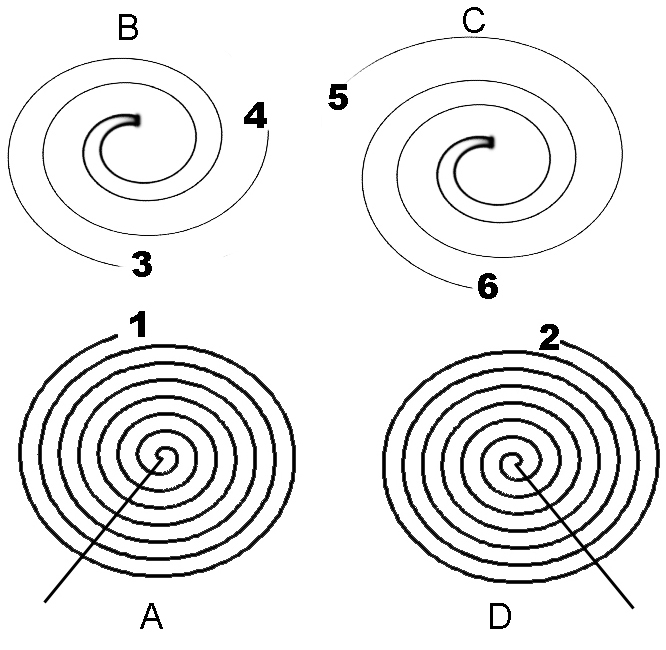
\includegraphics[width=5in]{TopN.jpg}
\caption{Illustrations of the TopN algorithms with top 4 subregions ($k=5$ and $N=4$).}
\label{TopN}
%\vspace*{-3ex}
\end{figure}

\begin{figure}
\noindent\fbox{%
\begin{minipage}{\dimexpr\linewidth-2\fboxsep-2\fboxrule\relax}
%\begin{algorithmic}[1]
Path TopN(Point start, Point end, int T, ArrayList centroids, ProbabilityMap map) \{ \\
\setlength\parindent{20pt}
1. Find closest centroid to start c1 and time needed t1  \\
2. Remove c1 from ArrayList centroids \\
3. Plan straight path from start to c1 and store in path1 \\
\indent map.VacuumProbability(path1); \\
4. Find closest centroid to end cN and time needed tN \\
5. Remove cN from ArrayList centroids \\
6. Plan straight path from end to cN and store in path2N \\
\indent map.VacuumProbability(path2N); \\
\indent int TLeft = T - t1 - tN; \\
\indent Path path2 = new Path(); \\
\indent Path path2.add(BestNeighbor(c1)); \\
\indent Path path2NMinus1 = new Path(); \\
\indent Path path2NMinus1.add(BestNeighbor(cN)); \\
\indent ArrayList segments = new ArrayList(); \\
\indent ArrayList segments.add(path2); \\
\indent ArrayList segments.add(path2NMinus1); \\
\indent foreach (Point c in centroids) \{ \\ 
\indent \indent	Path p1 = new path(); \\
\indent \indent p1.add(c); \\
\indent \indent Path p2 = new path(); \\
\indent \indent p2.add(BestNeighbor(c));\\
\indent \indent segments.add(p1); \\
\indent \indent segments.add(p2); \\
\indent \} \\
\indent while (EnoughTimeToJoinAllSegments(TLeft)) \{  \\
\indent \indent Path path = SegmentWithBestNeighbor(segments); \\
\indent \indent Point p = BestNeighbor(p.lastPoint()); \\
\indent \indent path.add(p); \\
\indent \indent map.VacuumProbability(p); \\
\indent \indent TLeft--; \\
\indent \} \\
\indent return JoinPaths(path1, path2N, segments);\\
\}
\end{minipage}% 
}
\caption{Pseudo-code for the TopN Algorithm with end point specified at one layer of the hierarchy (e.g., top 4 Gaussians out of 5).}
\label{Code2}
\end{figure}

%=================================================================================	
\section{Experiment Results and Analysis}
\label{sec:ExperimentResultsAndAnalysis}

%=============================
\subsection{Experiment Set Up}

We selected three real WiSAR scenarios to test the performance of the proposed algorithms for ecological validity. All three scenarios were obtained from George Mason University, and all came from the International Search and Rescue Incident Database (ISRID)~\cite{Koester2008Lost}. In each scenario, the missing person's Last Know Position (LKP) is at the center of a 2.4km$\times$2.4km search area, therefore, we always start the UAV path from the center of the map. The probability distribution map of the missing person for each scenario is generated using the Bayesian model presented in~\cite{Lin2010Bayesian}. These probability distribution maps have been evaluated at George Mason University's MapScore web portal~\cite{Twardy2012MapScore} and performed better than most other models evaluated\footnote{Scoring 0.8184, 0.9858, and 0.9892 on a [-1,1] scale where the higher the score the better. http://sarbayes.org/projects/}. The task-difficulty map for each scenario is built using vegetation density data downloaded from the USGS web site and categorized into three difficulty levels (sparse, medium, and dense). Although this method only considers the vegetation density, it gives us a reasonable task-difficulty map and serves well for the purpose of demonstrating algorithm performances\footnote{In real wilderness search and rescue operations, these maps would be further improved by domain experts before they are used for path planning.}. The probability distribution maps and the task-difficulty maps are discretized into 100$\times$100 grids. 

For each scenario, we compare the performance of the BA, LHC-GW-CONV, Top2, and TopN algorithms in $\mathit{Efficiency_{LB}}$ and running time for three flight durations ($T=300,600,900$, equivalent to 10, 20, and 30 minutes). Because we re-implemented the BA algorithm in MATLAB and the rest algorithms in C\#, for a fair comparison we omit the running time for the BA algorithm. We also present the performance of the Top2 and TopN algorithms for just one hierarchy layer to demonstrate that the two algorithms can achieve much better $\mathit{Efficiency_{LB}}$ in comparable running time with even arbitrary parameters ($k=5$ Gaussians and $N=3$ for top 3 subregions). In all the experiments we did not specify the ending location for the UAV because the BA algorithm does not support this feature. All the other algorithms, however, do support this feature.

Experiments were performed in simulated searches and not on-board real UAVs. All paths generated in the experiments were for a hexacopter although the algorithms also work for fixed-wing UAVs. All experiments were run on a Intel 4-core i7-2600 PC with 16GB of memory. For each scenario we ran 10 experiments and recorded the mean and standard deviation of $\mathit{Efficiency_{LB}}$ and running time. Due to space limitations, only a subset of the experiment results are presented.

%=============================
\subsection{Experiments Results and Analysis}

\begin{figure}
\centering
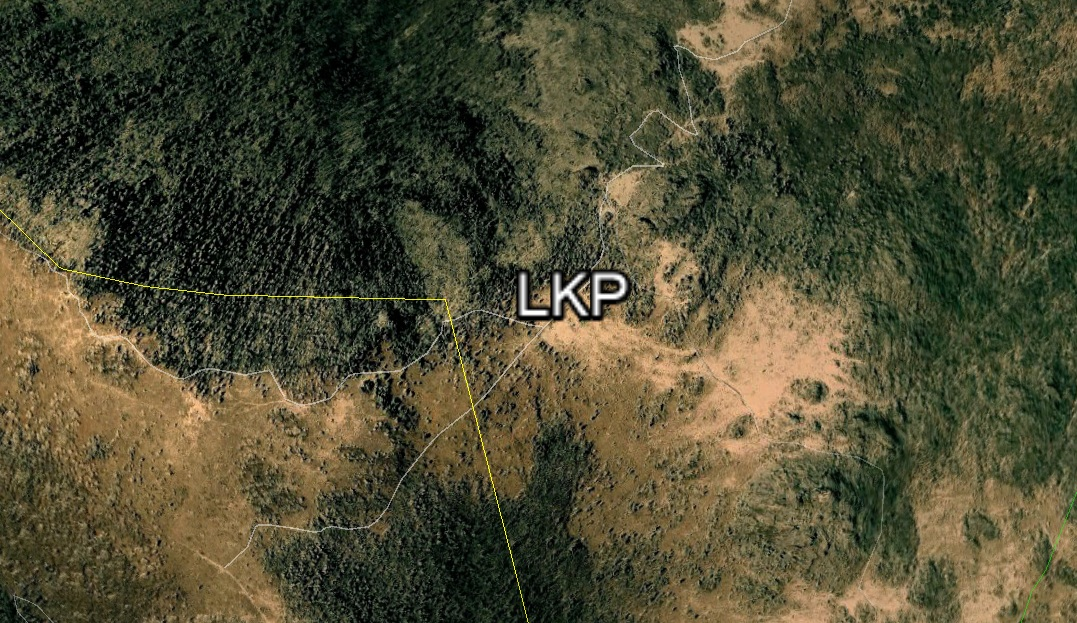
\includegraphics[width=6in]{HikerPaulSAT.jpg}
\caption{Satellite imagery of the search area for the HikerPaul scenario (near the Grayson Highlands State Park in Virginia) showing the vegetation density. The Last Known Position (LKP) of the missing person is at the center of the image.}
\label{HikerPaulSAT}
%\vspace*{-1ex}
\end{figure}

%=============
% HikerPaul
%=============
%In the first WiSAR scenario (HikerPaul), an elderly couple was reported missing near the Grayson Highlands State Park in Virginia. Fig.\ref{HikerPaulSAT} shows a satellite imagery of the search area for the scenario where the Last Known Position (LKP) of the missing person is in the center of the image. Fig.\ref{HikerPaulMaps} shows the probability distribution map (left) and the task difficulty map (middle) for the scenario. The right part of the figure shows the resulting surface when we combine the probability distribution map and the task difficulty map, which is the amount of probability the UAV can collect on its first visit to each vertex (or grid cell). The task difficulty map indicates that large areas of the search area were covered with dense vegetation, but there are also many small subregions with sparse vegetation (higher probability of detection).
%
%Fig.\ref{HikerPaulPaths} shows the paths generated by the BA, LHC-GW-CONV, Top2, and TopN algorithms. Both the BA and LHC-GW-CONV greedy-type algorithms generated paths that centered around the starting point and could not break away from the probability hills near the center of the search area. The Top2 algorithm, on the other hand, directed the UAV to cover the tall probability hill on the left side of the search area, and the TopN algorithm additionally directed the UAV to cover subregions in the lower right of the search area where more probability can be accumulated. Table~\ref{HikerPaul} shows the performance of the four algorithms and also the Top2 and TopN algorithms with specific parameters (Number of Gaussians to fit: $k=5$ and top $N$ subregions for TopN algorithm: $N=3$). The Top2 and TopN algorithms clearly outperform the BA and LHC-GW-CONV algorithms (whether using arbitrary parameters or search through the hierarchy) with significantly better $\mathit{Efficiency_{LB}}$. Searching through the hierarchy obviously generated more efficient paths than only working with one layer of the hierarchy. The TopN algorithm also achieved slightly better $\mathit{Efficiency_{LB}}$ than the Top2 algorithm. When using arbitrary parameters (only generating path for one layer of the hierarchy), both the Top2 and TopN algorithms are faster than the LHC-GW-CONV algorithm. When searching through the hierarchy, the Top2 and TopN algorithm did take a little bit longer, but still completed within 2 seconds.

In the first WiSAR scenario (HikerPaul), an elderly couple was reported missing near the Grayson Highlands State Park in Virginia (Fig.\ref{HikerPaulSAT} shows a satellite imagery of the search area for the scenario). In the second WiSAR scenario (NewYork53), a 46 year old male camper was reported missing near Adirondack Park in upper state New York. In the third WiSAR scenario (NewYork108), two teenage female hikers were reported missing near West Chesterfield in Massachusetts. For each scenario the Last Known Position (LKP) of the missing person is in the center of the search region. Fig.\ref{HikerPaulMaps}, \ref{NewYork53Maps} and \ref{NewYork108Maps} show the probability distribution map (left) and the task-difficulty map (middle) for these scenarios. The right part of the figure shows the resulting surface for each scenario when we combine the probability distribution map and the task-difficulty map, which is the amount of probability the UAV can collect on its first visit to each vertex (or grid cell). The task-difficulty maps indicate that large areas of these search regions were covered with dense vegetation, which makes detecting the missing person more difficult. There are also small subregions with sparse vegetation (higher probability of detection). Fig.\ref{HikerPaulPaths}, \ref{NewYork53Paths} and \ref{NewYork108Paths} show the paths generated by the BA, LHC-GW-CONV, Top2, and TopN algorithms for each scenario, respectively. The teleport paths for these scenario are not shown because they are mostly made up of disjointed points. Note that the paths sometimes revisit vertices that have already been visited (path segments cross with previous segments), but the combined surfaces we show in Fig.\ref{HikerPaulMaps}, \ref{NewYork53Maps} and \ref{NewYork108Maps} (right) only represent the amount of probability the UAV can collect on its first visit. Each surface is updated after each vertex visit to reflect the amount of probability collectable on the next visit.

%=============

\begin{figure}
\centering
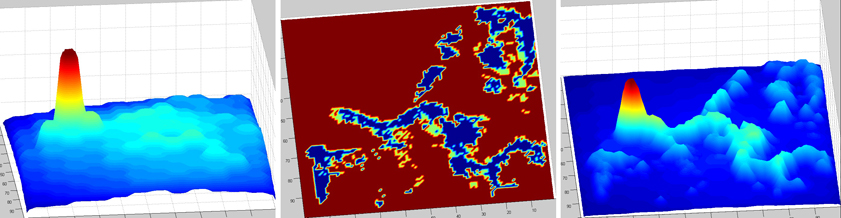
\includegraphics[width=6in]{HikerPaulMaps.jpg}
\caption{The HikerPaul scenario. Left: Probability distribution map. Middle: Task-difficulty map. Right: Surface after combining the probability distribution map and the task-difficulty map.}
\label{HikerPaulMaps}
%\vspace*{-2ex}
\end{figure}
\begin{figure}
\centering
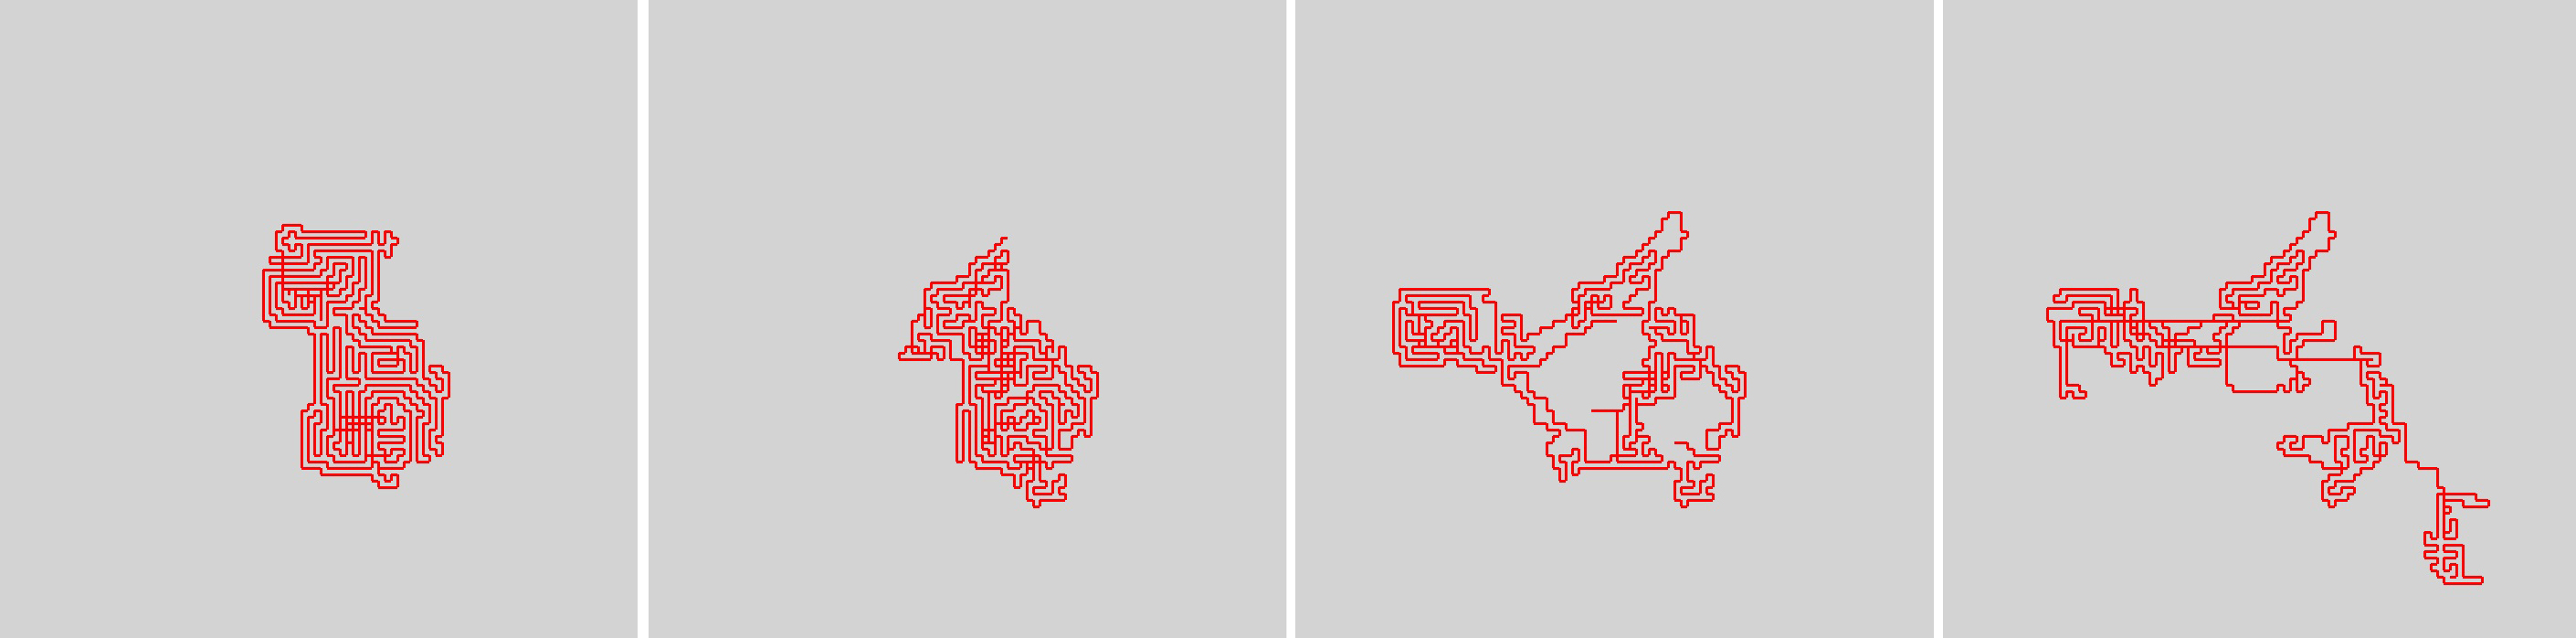
\includegraphics[width=6in]{HikerPaulPaths.jpg}
\caption{Paths generated for HikerPaul scenario with $T=900$ a) BA b) LHC-GW-CONV c) Top2 d) TopN}
\label{HikerPaulPaths}
%\vspace*{-2ex}
\end{figure}
\begin{figure}
\centering
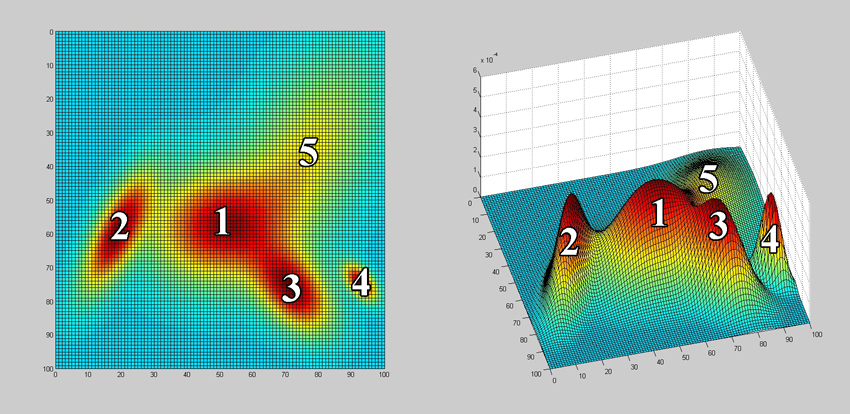
\includegraphics[width=6in]{GMM.jpg}
\caption{The Gaussian Mixture identified for the HikerPaul scenario with $T=900$ and $k=5$. The numbers show the ranking of the Gaussians using Mode Goodness Ratio. Left: Gaussians in 2D. Right: Gaussians in 3D.}
\label{GMMRanking}
%\vspace*{-2ex}
\end{figure}
\begin{table}
\caption{Algorithms $\mathit{Efficiency_{LB}}$ and running speed comparison for the HikerPaul scenario. All numbers shown are averages of 10 runs. All $\mathit{Efficiency_{LB}}$ standard deviations are below 0.1.}
%\small
	\centering
		\begin{tabular}
			{|l|c|c|c|c|c|c|}
			\hline
			 & \multicolumn{3}{|c|}{$\mathit{Efficiency_{LB}}$ (\%)} & \multicolumn{3}{|c|}{Speed (seconds)} \\
			\hline
			$T$ & 300 & 600 & 900	& 300 & 600 & 900 \\
			\hline
			BA & 56.95 & 60.07 & 57.11 & - & - & - \\
			\hline			
			LHC-GW-CONV & 60.18 & 56.76 & 55.18 & 0.30 & 0.47 & 0.98 \\
			\hline			
			Top2 (1 layer)	& 66.68 & 65.21 & 66.08 & \textbf{0.24} & 0.30 & 0.41 \\ 
			\hline
			TopN (1 layer)	& 76.19 & 71.02 & 68.26 & 0.25 & \textbf{0.24} & \textbf{0.22} \\ 
			\hline
			Top2 (Hierarchy) & 78.67 & 73.81 & 72.75 & 0.73 & 0.84 & 1.19 \\ 
			\hline
			TopN (Hierarchy) & \textbf{81.43} & \textbf{75.48} & \textbf{74.13} & 1.52 & 1.73 & 1.68 \\ 
			\hline			
		\end{tabular}
%\vspace*{2ex}
\label{HikerPaul}
%\vspace*{-2ex}
\end{table}

For the HikerPaul scenario, Fig.\ref{HikerPaulPaths} shows that both the BA and LHC-GW-CONV greedy-type algorithms generated paths that centered around the starting point and could not break away from the probability hills near the center of the search area. The Top2 algorithm, on the other hand, directed the UAV to cover the tall probability hill on the left side of the search area, and the TopN algorithm additionally directed the UAV to cover subregions in the lower right of the search area where more probability can be accumulated. Fig.\ref{GMMRanking} demonstrates how a GMM can be used to prioritize search subregions and shows the 5 Gaussians identified when we performed the Gaussian fitting for the HikerPaul scenario with $T=900$ and $k=5$. The Gaussians are ranked using the Mode Goodness Ratio heuristic values (1.39, 1.01, 1, 0.87, and 0.46 respectively). Table~\ref{HikerPaul} shows the performance of the four algorithms and also the Top2 and TopN algorithms with specific parameters (Number of Gaussians to fit: $k=5$ and top $N$ subregions for TopN algorithm: $N=3$). The Top2 and TopN algorithms clearly outperform the BA and LHC-GW-CONV algorithms (whether using arbitrary parameters or search through the hierarchy) with significantly better $\mathit{Efficiency_{LB}}$. Searching through the hierarchy generated more efficient paths than only working with one layer of the hierarchy. The TopN algorithm also achieved slightly better $\mathit{Efficiency_{LB}}$ than the Top2 algorithm. When using arbitrary parameters (only generating a path for one layer of the hierarchy), both the Top2 and TopN algorithms are faster than the LHC-GW-CONV algorithm. When searching through the hierarchy, the Top2 and TopN algorithm did take a little bit longer, but still completed within 2 seconds.

%=============
% NewYork53
%=============

%In the second WiSAR scenario (NewYork53), a 46 year old male camper was reported missing near Adirondack Park in upperstate New York. Fig.\ref{NewYork53Maps} shows the probability distribution map (left) and the task difficulty map (middle) for the scenario, and the surface when we combine the probability distribution map and the task difficulty map together (right), which is the amount of probability the UAV can collect on its first visit to each vertex (or grid cell). The task difficulty map indicates that the majority of the search area is covered by dense vegetation, which makes detecting the missing person more difficult.
%
%Fig.\ref{NewYork53Paths} shows the paths generated by the BA, LHC-GW-CONV, Top2, and TopN algorithms. Both the BA and LHC-GW-CONV greedy-type algorithms generated paths that spent a good amount of time right at the center of the search area around the starting point before sending the UAV to two other subregions on the right. The Top2 and TopN algorithms, however, did not waste any time at the center subregion and immediately directed the UAV to cover the two subregions on the right side of the search area. The TopN algorithm also directed the UAV to cover a subregion in the upper right part of the search area. Table~\ref{NewYork53} shows the performance of the four algorithms and also the Top2 and TopN algorithms with specific parameters ($k=5$ and $N=3$). The results show the same trend as with the first scenario where the Top2 and TopN algorithms outperform the BA and LHC-GW-CONV algorithms significantly in $\mathit{Efficiency_{LB}}$. Even with arbitrary parameters, the Top2 and TopN algorithms generated much more efficient paths (e.g., 59.15\% for TopN with one layer vs. BA with 39.95\%). The TopN algorithm also outperformed Top2 algorithm in $\mathit{Efficiency_{LB}}$. When looking at the algorithm completion time, LHC-GW-CONV algorithm is the clear winner in this scenario. When arbitrary parameters are used, the Top2 and TopN algorithms both completed within 1 second, but when searching through the hierarchy, both algorithms took much longer (about 2 seconds for TopN and 6 seconds for TopN) to complete.

%=============

\begin{figure}
\centering
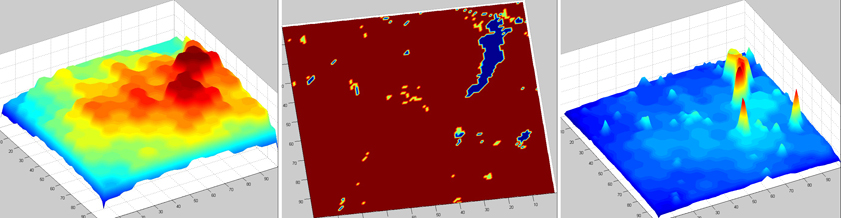
\includegraphics[width=6in]{NewYork53Maps.jpg}
\caption{The NewYork53 scenario. Left: Probability distribution map. Middle: Task-difficulty map. Right: Surface after combining the probability distribution map and the task-difficulty map.}
\label{NewYork53Maps}
%\vspace*{-2ex}
\end{figure}
\begin{figure}
\centering
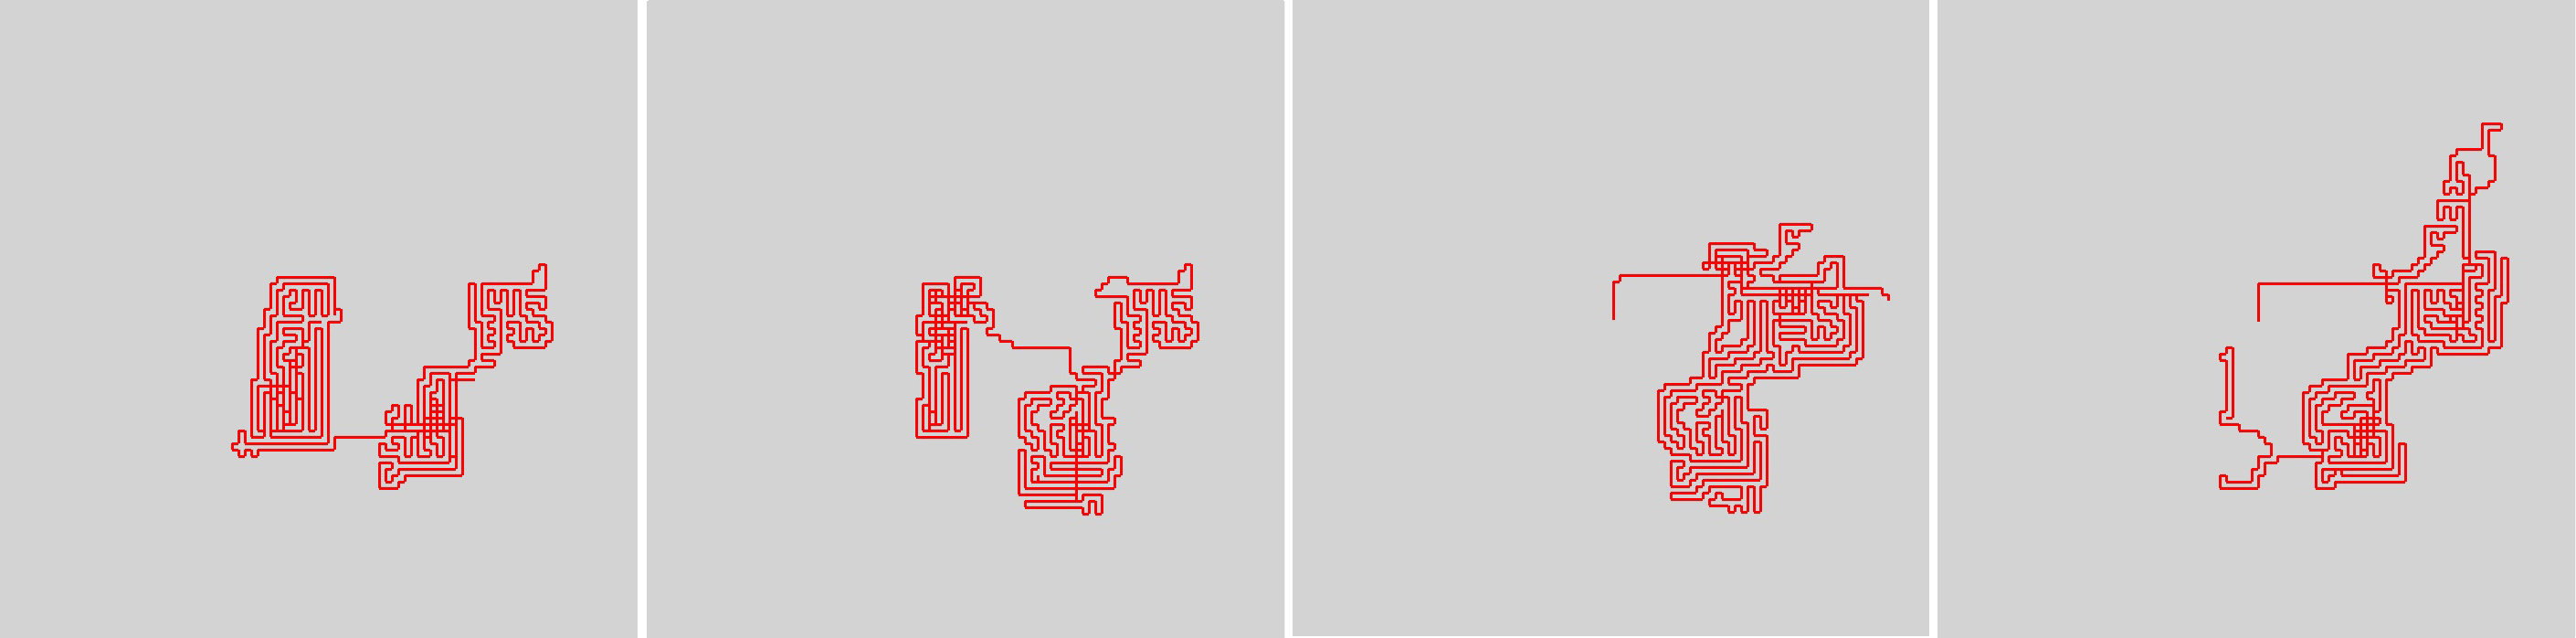
\includegraphics[width=6in]{NewYork53Paths.jpg}
\caption{Paths generated for NewYork53 scenario with $T=900$ a) BA b) LHC-GW-CONV c) Top2 d) TopN}
\label{NewYork53Paths}
%\vspace*{-2ex}
\end{figure}
\begin{table}
\caption{Algorithms $\mathit{Efficiency_{LB}}$ and running speed comparison for the NewYork53 scenario. All numbers shown are averages of 10 runs. All $\mathit{Efficiency_{LB}}$ standard deviations are below 0.07.}
%\small
	\centering
		\begin{tabular}
			{|l|c|c|c|c|c|c|}
			\hline
			 & \multicolumn{3}{|c|}{$\mathit{Efficiency_{LB}}$ (\%)} & \multicolumn{3}{|c|}{Speed (seconds)} \\
			\hline
			$T$ & 300 & 600 & 900	& 300 & 600 & 900 \\
			\hline
			BA & 39.95 & 54.27 & 65.08 & - & - & - \\
			\hline			
			LHC-GW-CONV & 38.47 & 56.91 & 67.38 & \textbf{0.01} & \textbf{0.02} & \textbf{0.02} \\
			\hline			
			Top2 (1 layer)	& 54.42 & 66.61 & 72.79 & 0.75 & 0.92 & 0.81 \\ 
			\hline
			TopN (1 layer)	& 59.15 & 68.78 & 74.54 & 0.70 & 0.77 & 0.69 \\ 
			\hline
			Top2 (Hierarchy) & 57.18 & 69.29 & 74.44 & 1.87 & 2.06 & 1.92 \\ 
			\hline
			TopN (Hierarchy) & \textbf{65.39} & \textbf{71.47} & \textbf{77.36} & 5.01 & 5.76 & 5.32 \\ 
			\hline			
		\end{tabular}
%\vspace*{2ex}
\label{NewYork53}
%\vspace*{-2ex}
\end{table}

For the NewYork53 scenario, Fig.\ref{NewYork53Paths} shows that both the BA and LHC-GW-CONV greedy-type algorithms generated paths that spent a good amount of time right at the center of the search area around the starting point before sending the UAV to two other subregions on the right. The Top2 and TopN algorithms, by contrast, did not waste any time at the center subregion and immediately directed the UAV to cover the two subregions on the right side of the search area. The TopN algorithm also directed the UAV to cover a subregion in the upper right part of the search area. Table~\ref{NewYork53} shows the performance of the four algorithms and also the Top2 and TopN algorithms with specific parameters ($k=5$ and $N=3$). The results show the same trend as with the first scenario where the Top2 and TopN algorithms outperform the BA and LHC-GW-CONV algorithms significantly in $\mathit{Efficiency_{LB}}$. Even with arbitrary parameters, the Top2 and TopN algorithms generated much more efficient paths (e.g., 59.15\% for TopN with one layer vs. BA with 39.95\%). The TopN algorithm also outperformed Top2 algorithm in $\mathit{Efficiency_{LB}}$. When looking at the algorithm completion time, LHC-GW-CONV algorithm is the clear winner in this scenario. When arbitrary parameters are used, the Top2 and TopN algorithms both completed within 1 second, but when searching through the hierarchy, both algorithms took much longer (about 2 seconds for Top2 and 6 seconds for TopN) to complete.

%=============
% NewYork108
%=============

%In the third WiSAR scenario (NewYork108), two teenage female hikers were reported missing near West Chesterfield in Massachusetts. Fig.\ref{NewYork108Maps} shows the probability distribution map (left) and the task difficulty map (middle) for the scenario, and the surface when we combine the probability distribution map and the task difficulty map together (right). The task difficulty map shows that large areas of the search area are covered by dense vegetation, which makes the search more difficult.
%
%Fig.\ref{NewYork108Paths} shows the paths generated by the BA, LHC-GW-CONV, Top2, and TopN algorithms. Both the BA and LHC-GW-CONV greedy-type algorithms generated paths that spent a good amount of time at the center of the search area around the starting point before moving on to the upper right subregion of the search area to cover the probability ridge. The Top2 and TopN algorithms, however, did not waste any time at the center subregion and immediately directed the UAV to cover the probability ridge at the upper right subregion of the search area. Both of them also sent the UAV to another subregion at the lower left part of the search area where a good amount of probability can be collected. Table~\ref{NewYork108} shows the performance of the four algorithms and also the Top2 and TopN algorithms with specific parameters ($k=5$ and $N=3$). The results show the same trend as with the previous two scenarios where the Top2 and TopN algorithms outperform the BA and LHC-GW-CONV algorithms significantly in $\mathit{Efficiency_{LB}}$. Even with arbitrary parameters, the Top2 and TopN algorithms generated more efficient paths (e.g., 58.37\% for Top2 with one layer vs. BA with 39.92\%). In this scenario, the Top2 algorithm performed slighly better than the TopN algorithm in $\mathit{Efficiency_{LB}}$ at $T=300$ (60.73\% for Top2 and 59.60\% for TopN), but the TopN algorithm performed much better than the Top2 algorithm for the other two cases. When looking at the algorithm completion time, LHC-GW-CONV algorithm is still the clear winner in this scenario. When arbitrary parameters are used, the Top2 and TopN algorithms both completed in about 1 second, but when searching through the hierarchy, both algorithms took much longer (about 2.5 seconds for TopN and 7 seconds for TopN) to complete.

%=============

\begin{figure}
\centering
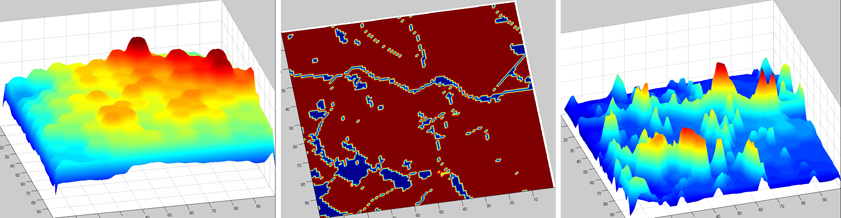
\includegraphics[width=6in]{NewYork108Maps.jpg}
\caption{The NewYork108 scenario. Left: Probability distribution map. Middle: Task-difficulty map. Right: Surface after combining the probability distribution map and the task-difficulty map.}
\label{NewYork108Maps}
%\vspace*{-2ex}
\end{figure}
\begin{figure}
\centering
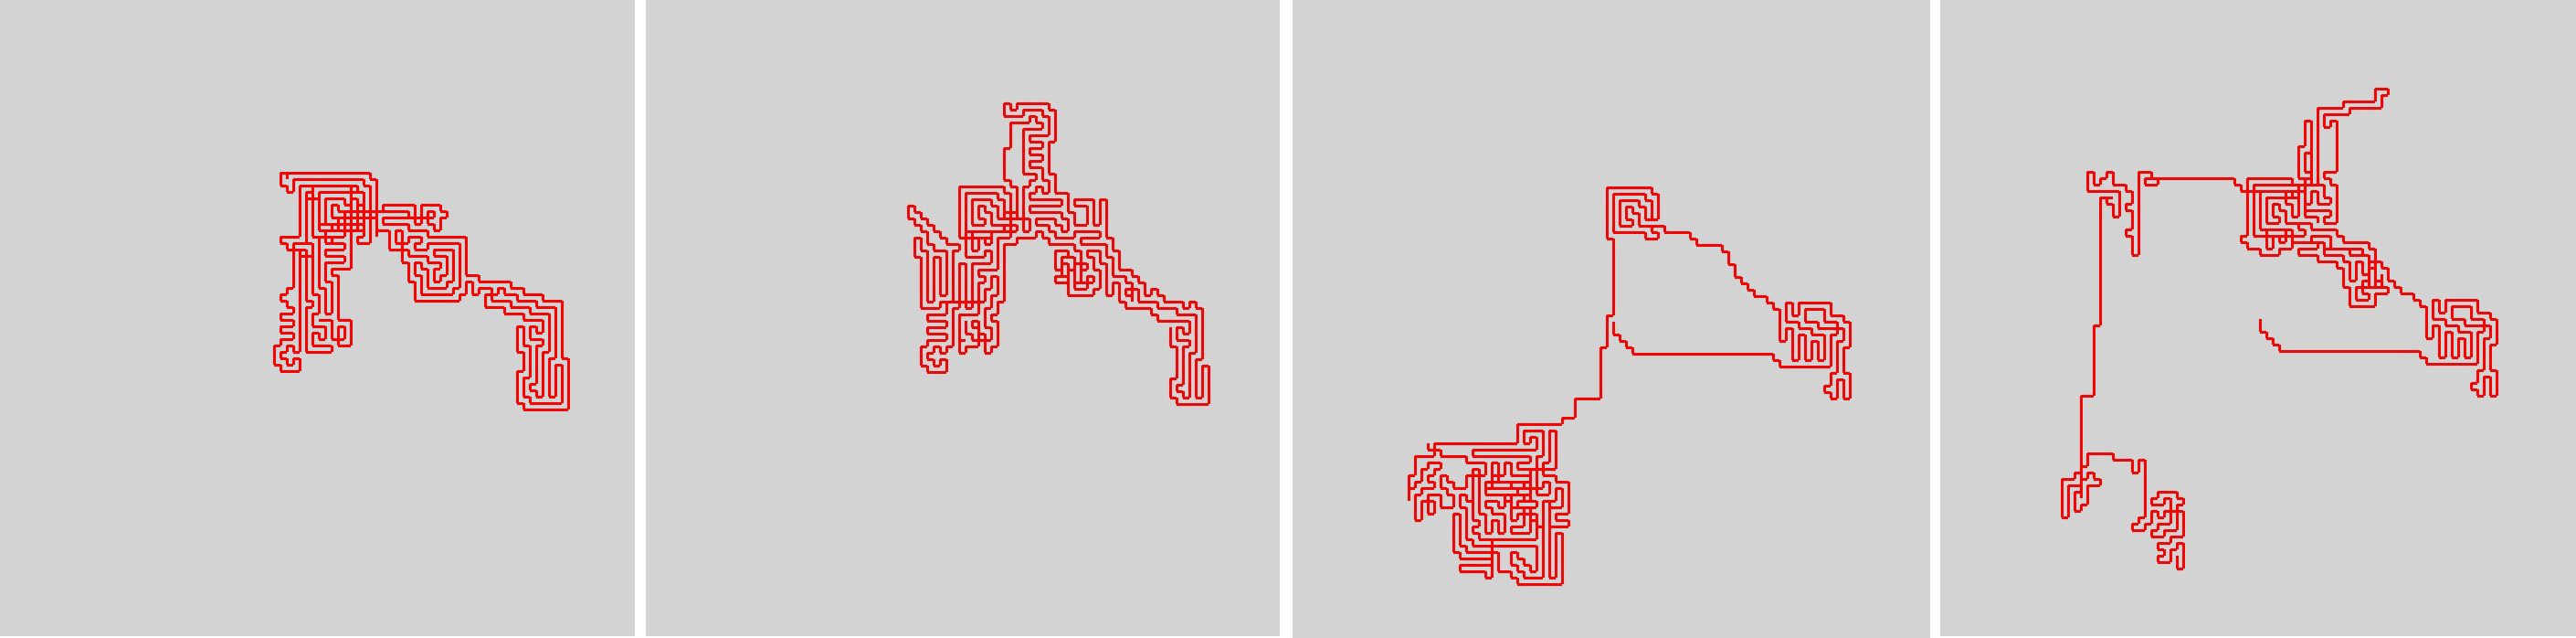
\includegraphics[width=6in]{NewYork108Paths.jpg}
\caption{Paths generated for NewYork108 scenario with $T=900$ a) BA b) LHC-GW-CONV c) Top2 d) TopN}
\label{NewYork108Paths}
%\vspace*{-2ex}
\end{figure}
\begin{table}
\caption{Algorithms $\mathit{Efficiency_{LB}}$ and running speed comparison for the NewYork108 scenario. All numbers shown are averages of 10 runs. All $\mathit{Efficiency_{LB}}$ standard deviations are below 0.07.}
%\small
	\centering
		\begin{tabular}
			{|l|c|c|c|c|c|c|}
			\hline
			 & \multicolumn{3}{|c|}{$\mathit{Efficiency_{LB}}$ (\%)} & \multicolumn{3}{|c|}{Speed (seconds)} \\
			\hline
			$T$ & 300 & 600 & 900	& 300 & 600 & 900 \\
			\hline
			BA & 39.92 & 45.34 & 49.39 & - & - & - \\
			\hline			
			LHC-GW-CONV & 41.38 & 52.88 & 52.61 & \textbf{0.01} & \textbf{0.01} & \textbf{0.02} \\
			\hline			
			Top2 (1 layer)	& 58.37 & 54.18 & 57.33 & 0.98 & 0.90 & 1.44 \\ 
			\hline
			TopN (1 layer)	& 54.03 & 53.91 & 57.91 & 0.92 & 0.83 & 0.97 \\ 
			\hline
			Top2 (Hierarchy) & \textbf{60.73} & 55.91 & 57.94 & 2.42 & 2.52 & 2.50 \\ 
			\hline
			TopN (Hierarchy) & 59.60 & \textbf{60.26} & \textbf{60.99} & 6.81 & 6.59 & 7.42 \\ 
			\hline			
		\end{tabular}
%\vspace*{2ex}
\label{NewYork108}
%\vspace*{-2ex}
\end{table}

For the NewYork108 scenario, Fig.\ref{NewYork108Paths} shows that both the BA and LHC-GW-CONV greedy-type algorithms generated paths that spent a good amount of time at the center of the search area around the starting point before moving on to the upper right subregion of the search area to cover the probability ridge. The Top2 and TopN algorithms, however, did not waste any time at the center subregion and immediately directed the UAV to cover the probability ridge at the upper right subregion of the search area. Both of them also sent the UAV to another subregion at the lower left part of the search area where a good amount of probability can be collected. Table~\ref{NewYork108} shows the performance of the four algorithms and also the Top2 and TopN algorithms with specific parameters ($k=5$ and $N=3$). The results show the same trend as with the previous two scenarios where the Top2 and TopN algorithms outperform the BA and LHC-GW-CONV algorithms significantly in $\mathit{Efficiency_{LB}}$. Even with arbitrary parameters, the Top2 and TopN algorithms generated more efficient paths (e.g., 58.37\% for Top2 with one layer vs. BA with 39.92\%). In this scenario, the Top2 algorithm performed slighly better than the TopN algorithm in $\mathit{Efficiency_{LB}}$ at $T=300$ (60.73\% for Top2 and 59.60\% for TopN), but the TopN algorithm performed much better than the Top2 algorithm for the other two cases. When looking at the algorithm completion time, LHC-GW-CONV algorithm is still the clear winner in this scenario. When arbitrary parameters are used, the Top2 and TopN algorithms both completed in about 1 second, but when searching through the hierarchy, both algorithms took much longer (about 2.5 seconds for Top2 and 7 seconds for TopN) to complete.

%=============

Note that the performance metric $\mathit{Efficiency_{LB}}$ is computed using Equation~\ref{EfficiencyLB}, which assumes that the UAV can teleport within the search area. Because the amount of probability accumulated following this teleporting path can be much better than the optimal path, the true search efficiency is likely much better than the value of the $\mathit{Efficiency_{LB}}$. Fig.\ref{CDPGraph} shows the comparison of the algorithms performance with respect to CDP collected over time for the NewYork53 scenario when $T=900$. The dotted red line represents CDP accumulated over time if the UAV could teleport from vertex to vertex. Therefore this line represents the theoretical CDP upperbound. If we know the optimal path and can plot the performance, that line would most likely be somewhere below the teleport path line. The TopN algorithm (black solid line) performed the best (highest CDP value at time step 900), and the Top2 algorithm (blue dash line) ranked second. Both the Top2 and TopN algorithms outperformed the BA and LHC-GW-CONV algorithms (the bottom two dashed lines) significantly.

Across experiments, results show that by taking advantage of the Mode Goodness Ratio heuristic, the Top2 and TopN algorithms (even when arbitrary parameters, $k=5$ Gaussians to fit and $N=3$ for top 3 subregions, are used) always generated more efficient paths than those generated by the BA and LHC-GW-CONV algorithms. When hierarchical search is performed, the improvement from Top2 and TopN algorithms is significant. In most cases, the TopN algorithm outperformed the Top2 algorithm. However, when hierarchical search is performed, the Top2 and TopN algorithms did take a little longer to complete.
\begin{figure}
\centering
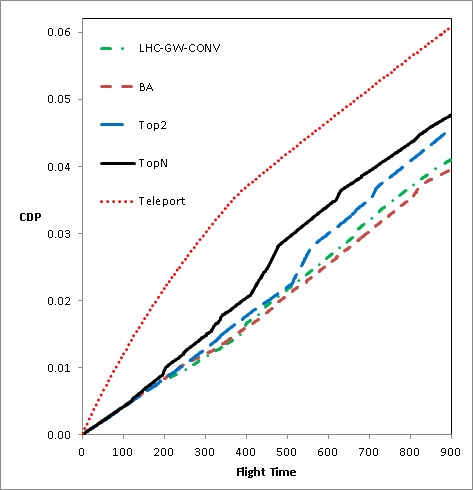
\includegraphics[width=6in]{CDPGraph.jpg}
\caption{Paths CDPs comparison at $T$=900 with partial detection.}
\label{CDPGraph}
%\vspace*{-3ex}
\end{figure}


%For example, Fig.\ref{GaussianFitting} Middle shows the Gaussian fitting result for the multimodal distribution map. At $T$=900, mode 1, 2, and 3 have the best Mode Goodness Ratio (at 1.796, 1, and 0.757 respectively). The path created by the TopN algorithm focus on these three subregions and outperformed the other two algorithms with a $\mathit{Efficiency_{LB}}$ at 89.53\%.

%\begin{figure}
%\centering
%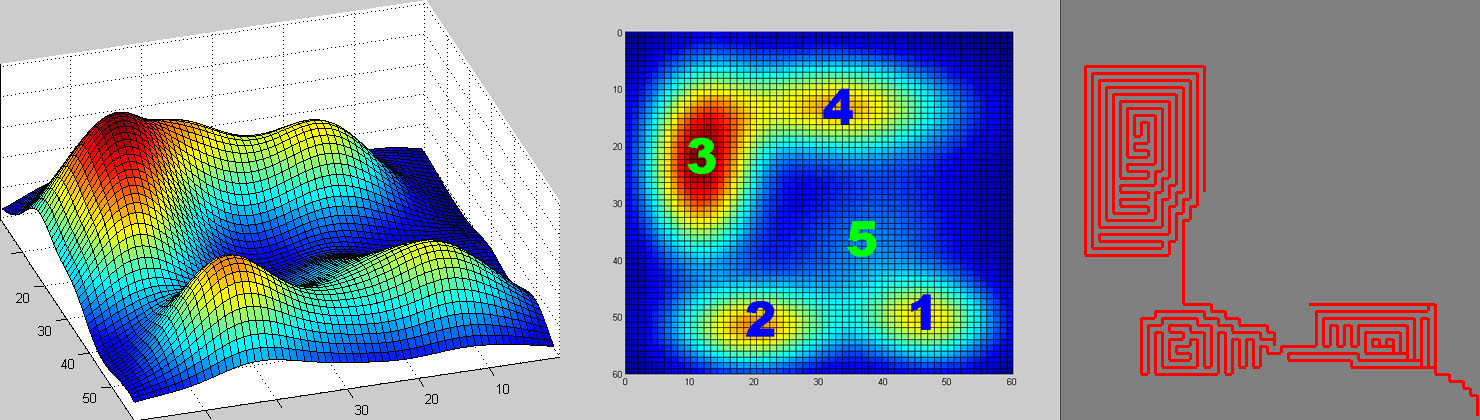
\includegraphics[width=3.2in]{GaussianFitting.jpg}
%\caption{Left: Multimodal probability distribution. Middle: Result of Gaussian fitting. Right: Path created by TopN at $T$=900.}
%\label{GaussianFitting}
%\end{figure}

%=================================================================================	
\section{Limitations and Discussion}
\label{sec:LimitationsAndDiscussion}

In our problem formulation, we treat the missing person as stationary because the speed of the missing person in wilderness is relatively low when compared with the speed the UAV travels in. False detection is not an issue because the UAV can simply follow the path generated to continuously collect detection probability while human operators verify the accuracy of the detection. For other application domains where the target might be moving or the probability distribution might be changing during search, by setting $T$ to a small value, we can easily adapt the Top2 and TopN algorithms to handle these situations. The two algorithms effectively turn into greedy (a $T$-step look ahead approach compared to the one-step look ahead method in~\cite{Bourgault2006Optimal}) algorithms with flexible time horizons and scalability. We leave the evaluation of the two algorithms in such scenarios to future work.

In Equation~\ref{NoDetection}, we assume that each observation at vertex $v_i$ is conditionally independent of each other. This assumption certainly has its limitation. If the environment features remain the same (e.g., lighting conditions, vegetation density) and the sensor platform (e.g., camera) has stable performance, then a high probability of no detection on the first visit might indicate high probability of no detection on future visits. However, in practical applications, a sensor operator's ability to recognize the missing person from video footprint is affected by many factors such as his fatigue level and his cognitive workload~\cite{Goodrich2008Supporting}, especially when the sensor operator might also be in charge of flying the UAV. In this case, the operator's chance performance can be regarded as independent trials (as in successive coin tosses).

The detection model used in our experiments is a simple decay model only parameterized by a difficulty factor. In SAR (Search and Rescue) literature, the parameters of the decay factor could be affected by environment features and sensor properties (e.g., distance to radar, signal strength~\cite{Bourgault2006Optimal}). Also we only consider vegetation density when we constructed the task-difficulty maps. Because we use a camera sensor and keep the UAV flying at the same height above ground, we believe this model is sufficient to show the algorithms' capability in handling partial detection, and we intentionally kept the sensor model and environment model simple for demonstration purposes. However, a more complicated sensor model and environement model can easily be applied to the system. 

Although GMM is a statistically mature method for clustering, it has several limitations. First, convergence is not guaranteed for the iterative EM algorithm used to estimate the Gaussian mixture. In our implementation, we re-run GMM multiple times if convergence is not achieved to overcome the problem. Second, how many Gaussians should we fit? There is the possibility that the Gaussians might not fit the data very well. We arbitrarily set the maximum Gaussians to 5 to reduce computational complexity. Experiment results show that we were still able to generate good paths. Since the Mode Goodness Ratio is only a heuristic, as long as it provides useful information to our search most of the time, it serves its purpose.

Another limitation is that the algorithms do not handle tough terrains where the UAV might not be able to climb fast enough to fly over the terrain. Future work should explore how to modify the algorithms to consider such constraints and actual flight dynamics.

When defining the goodness of a subregion, $MG_i$, we considered three factors: distance ratio, probability volume, and subregion area. The last two factors, when combined, give us a sense of the peakedness of a probability hill. Then we multiply the peakedness with the distance ratio in order to compare the Mode Goodness of subregions. Here we assume the two measures are independent of each other, which is a limitation of the heuristic. It also creates a trade off problem. For example, when subregion A's distance ratio is half of that of subregion B but A's peakedness is twice in size compared to B. A and B would still have identical $MG_i$ values. Should they be? We leave this to future work.

Going back to the synthetic scenario we presented in section~\ref{BALHCReview}, Table~\ref{Synthetic} shows the performance of the BA, LHC-GW-CONV, Top2, and TopN algorithms in two different scenarios: starting from a subregion with low task-difficulty (upper left) and starting from a subregion with high task-difficulty (lower right). When starting from a high task-difficulty area, the BA and LHC-GW-CONV algorithms tend to get stuck in a local probability hill, while the Top2 and TopN algorithms force the UAV to visit other subregions, therefore achieving better paths with significant improvement. One interesting observation we noticed is that if an ending position is specified for the desired UAV path and the ending point is in a subregion with low task-difficulty, the LHC-GW-CONV algorithm also forces the UAV to visit other subregions, and by doing so, improve the efficiency of the path. Fig.\ref{SyntheticCasePaths3} shows an example where the path on the right achieved 93.60\% in $\mathit{Efficiency_{LB}}$ (computed within 0.01 second), which is slightly better than the Top2 algorithm but not as good as the TopN algorithm. Another thing to note with this scenario is that the LHC-GW-CONV algorithm actually did slightly better than the Top2 and TopN algorithms when the UAV starts from a low task-difficulty area. We have noticed from various experiments that after combining the probability distribution map and the task-difficulty map, if the resulting surface is not a complicated one (meaning it only has a few distinctive probability hills), the LHC-GW-CONV algorithm generally performs well. For more complicated surfaces (such as the three real WiSAR scenarios we tested the algorithms with), the Top2 and TopN algorithms are more reliable in generating good UAV paths. 

%For scenarios where the probability distribution map is a mixture of Gaussians to start with and when the task difficulty map is uniform (with only 1 task difficulty level), the LHC-GW-CONV algorithm makes a good candidate. 

\begin{figure}
\centering
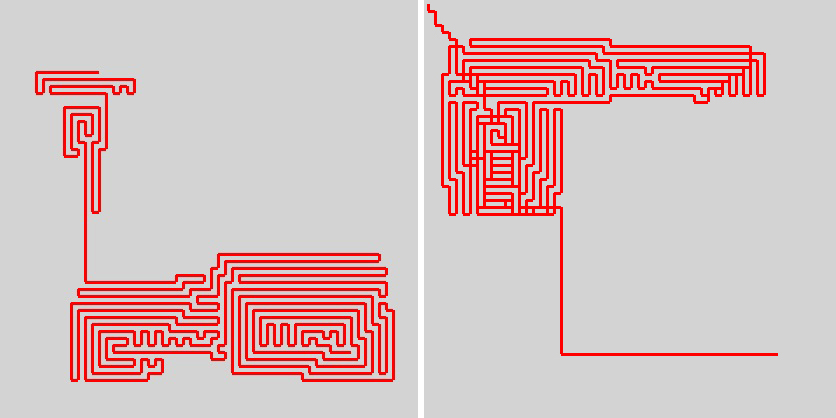
\includegraphics[width=5in]{TestCaseBottomRightWithEnd.jpg}
\caption{Paths found for the synthetic scenario at $T=900$ when the UAV starts from a subregion with high task-difficulty (lower right corner). Left: Path created by LHC-GW-CONV without specifying end point. Right: Path created by LHC-GW-CONV with specified end point at upper left corner.}
\label{SyntheticCasePaths3}
%\vspace*{-3ex}
\end{figure}

%In real WiSAR operations, if additional computation time is available, then the Top2 and TopN algorithms can search through the hierarchy to generate the best paths possible. If intant feedback is required in path planning, then Top2 and TopN algorithms with arbitrary parameters can be used, which still generate better paths than the BA and LHC-GW-CONV algorithms. Wolpert and Macready's famous No Free Lunch Theorem~\cite{wolpert1997no} basically states that no algorithm will always perform well in all state spaces. Therefore, a better approach is actually to run multiple algorithms in the same path planning task and then pick the one that performed the best. Since all these algorithms can finish within a few seconds, we can make them all seed algorithms in the Evolution Algorithm described in~\cite{lin2009uav} and try to come up with even better paths. 

In the current implementation, we used a grid representation for the probability distribution map, task-difficulty map, and the path generated. However, the algorithms also support other tessellation methods such as a hexagonal tessellation.
\begin{table}
\caption{Algorithms $\mathit{Efficiency_{LB}}$ comparison for the multi-modal synthetic scenario at $T=900$}
%\small
	\centering
		\begin{tabular}
			{|l|c|c|c|c|c|}
			\hline
			(\%) & BA & LHC-GW-CONV & Top2 & TopN \\
			\hline
			Start from upper left & 65.99 & \textbf{96.28} & 94.96 & 95.82 \\
			\hline			
			Start from lower right & 41.91 & 53.71 & 93.46 & \textbf{95.29} \\			\hline			
		\end{tabular}
%\vspace*{2ex}
\label{Synthetic}
%\vspace*{-3ex}
\end{table}

%=================================================================================	
\section{Summary} 
\label{sec:Summary}

We proposed a new heuristic, the Mode Goodness Ratio, which uses Gaussian Mixture Model to prioritize search subregions, and presented two new algorithms that utilize the heuristic in hierarchical path planning. The hierarchical structure enables searching for better paths through the parameter space at different scales and enables us to parallelize the two algorithms for better performance. The probability of detecting the desired subject based on UAV sensor information can vary in different search areas due to factors such as varying vegetation density or lighting conditions. We represented this type of partial detection in the form of a task-difficulty map, a spatial representation of sensor detection probability, and incorporate it into UAV path planning. We compared the performance of the new algorithms against two published algorithms BA and LHC-GW-CONV in simulated searches with three real search and rescue scenarios. Experiment results showed that by using the Mode Goodness Ratio heuristic, the two new algorithms Top2 and TopN consistently outperform the BA and LHC-GW-CONV algorithms, yielding efficient paths that produce payoff approximating the payoff of the optimal path.  
